\chapter{Linear Differential Equations}
\label{C:LDE}

\normalsize

Primarily our discussions of differential equations have focused on 
two issues: generalizations of solutions of the differential equation 
$\dot{x}=\lambda x$ to systems of equations and the qualitative 
interpretation of numerically obtained phase portraits for autonomous
nonlinear systems.   Except for finding closed form solutions of 
systems of equations $\dot{X}=AX$ (in the plane, Chapter~\ref{Chap:Planar}, 
or in Jordan normal form, Section~\ref{sec:LinHomSys}), we have solved in 
closed form virtually no other differential equation.  In this chapter and 
the next two we focus on finding closed form solutions to a variety of 
differential equations.  This chapter and the next discuss constant 
coefficient linear equations, both homogeneous and inhomogeneous, 
while Chapter~\ref{chap:SingleOdes} discusses nonconstant coefficient
and nonlinear equations.  

The system of differential equations $\dot{X}=AX$ is a constant coefficient, 
first order, homogeneous, linear system of ordinary differential equations. 
We begin this chapter (Section~\ref{S:SEOC}) by discussing how to solve 
the systems $\dot{X}=AX$ in the given coordinates (rather than by first 
transforming $A$ to Jordan normal form, as we did in 
Section~\ref{sec:LinHomSys}).  For example, we present a formula for 
computing $e^{tA}$ for any matrix $A$.  Later we solve some linear 
equations that are neither homogeneous nor first order.   

In Section~\ref{sec:HighOrder} we discuss how to solve higher order 
linear differential equations by reducing them to first order systems.  
This section generalizes the reduction of second order equations to planar
systems described in Section~\ref{S:SOE}.  We will see that generally it is 
easier to solve higher order equations in closed form than to solve first 
order systems.  Section~\ref{sec:2norderinhom} discusses the solution of an 
inhomogeneous higher order equation by undetermined coefficients.  The method 
of undetermined coefficients is most easily understood in the language of 
linear differential operators, and this language is introduced in 
Section~\ref{S:LDO}.

The chapter ends with a discussion of resonance in Section~\ref{S:resonance}. 
Here we use explicit closed form solutions found by the method of 
undetermined coefficients to understand a physically motivated phenomenon 
that occurs in solutions to forced second order equations.  


\Section{Solving Systems in Original Coordinates}
\label{S:SEOC}

In Section~\ref{sec:LinHomSys} we discussed one method for solving systems of 
first order constant coefficient linear differential equations.   We saw that 
such systems can be solved by putting the coefficient matrix $A$ in Jordan 
normal form and then computing the exponential of the Jordan normal form 
matrix.  

In this section we describe a second and a third approach to solving linear 
systems; the second method is based on finding the generalized eigenvectors 
that put $A$ into Jordan normal form\index{Jordan normal form} and then
computing solutions directly using this information while the third method is 
based on deriving a formula for the exponential\index{matrix!exponential} 
$e^{tA}$ in original coordinates.  The advantage of the second method is
that it is not necessary to perform the similarity that transforms the matrix 
$A$ to Jordan normal form and the advantage of the third method is that it is 
not necessary even to compute the eigenvectors of $A$.  Be forewarned,
however, that all of these methods require substantial calculations.

Let $A$ be an $n\times n$ matrix.  All methods for solving the system 
\begin{equation} \label{dotX=AX}
\dot{X}=AX
\end{equation}
begin by finding the eigenvalues\index{eigenvalue} of $A$.  This can be done 
either analytically (sometimes) or numerically (using \Matlabp). Then the  
methods diverge.  In the first and second methods, we need to find the 
eigenvectors and, if need be, the generalized eigenvectors
\index{eigenvector!generalized} of $A$; while in the third method, we need to 
perform tedious calculations involving partial fractions and matrix 
multiplications.  With either method, the calculations simplify enormously 
when the eigenvalues are simple.  Indeed, this simplification also occurs in 
the Jordan normal form method of Section~\ref{sec:LinHomSys}.

\subsection*{A Method Based on Eigenvectors}
 
In this method we find a basis for solutions of \Ref{dotX=AX}.  First, we 
review the simpler case when there is a basis of eigenvectors and then we 
consider (part of) the case when there is a deficiency of eigenvectors.

\subsubsection*{A Complete Set of Eigenvectors}

The simplest case in solving \Ref{dotX=AX} occurs when $A$ has a basis of 
eigenvectors $v_1,\ldots,v_n$ corresponding to the (not necessarily distinct) 
eigenvalues $\lambda_1,\ldots,\lambda_n$.  We showed how to find a basis for
the solutions of \Ref{dotX=AX} in Section~\ref{S:TDM} but review the results
here.  Each eigenvector $v_j$ generates the solution 
$X_j(t)=e^{\lambda_j t}v_j$ to \Ref{dotX=AX} and the general solution is:
\begin{equation} \label{E:gensolns}
X(t) = \alpha_1 X_1(t) + \cdots + \alpha_nX_n(t),
\end{equation}
where the scalars $\alpha_j$ are real when $\lambda_j$ is real and complex
when the $\lambda_j$ is not real.  

The initial value problem\index{initial value problem} is then solved 
by finding scalars $\alpha_j$ so that
\begin{equation}  \label{E:gensolnsic}
X_0 = X(0) =\alpha_1v_1 + \cdots + \alpha_nv_n.
\end{equation}
The solution of \Ref{E:gensolnsic} is a well understood linear algebra 
problem.   

\subsubsection*{Complex Eigenvalues}

The only complication occurs when some of the eigenvalues are complex. 
If $\lambda$ is a complex eigenvalue of the real matrix $A$, so is 
$\overline{\lambda}$.  If $v$ is a complex eigenvector corresponding to 
$\lambda$, then $\overline{v}$ is the complex eigenvector corresponding to 
$\overline{\lambda}$.  With this choice of eigenvector, $\overline{\alpha}$ 
is the scalar corresponding to the eigenvector $\overline{v}$ where $\alpha$
is the scalar corresponding to the eigenvector $v$.

More precisely, let $\lambda = \sigma+i\tau$ be an eigenvalue of $A$ and 
let $v=u+iw$ be a corresponding eigenvector.  We claim that 
\begin{equation}  \label{eq:reimsol}
X_1(t) = e^{\sigma t}(\cos(\tau t)u - \sin(\tau t)w)\quad
\mbox{and}\quad
X_2(t) = e^{\sigma t}(\sin(\tau t)u + \cos(\tau t)w)
\end{equation}
are solutions of the homogeneous equation \Ref{dotX=AX}.  Verifying that
$X_1$ and $X_2$ are solutions proceeds as follows.  The solutions 
corresponding to the eigenvalue $\lambda$ are 
\[
\alpha e^{\lambda t}v + \overline{\alpha} e^{\overline{\lambda}t}\overline{v}
= 2\RE\left(\alpha e^{\lambda t}v\right)
\]
for all complex scalars $\alpha$.  If we set $\alpha=\frac{1}{2}$, then 
using Euler's formula, we obtain the solution 
\[
\RE\left(e^{\lambda t}v\right) = e^{\sigma t}\RE\left((\cos(\tau t)+i\sin(\tau t))(u + iw)\right)=X_1(t)
\]
Similarly, setting $\alpha=-\frac{1}{2}i$ leads to the solution $X_2(t)$.  


\subsubsection*{Two Examples with a Complete Set of Eigenvectors}

Next we consider two examples.  The first has distinct eigenvalues, some 
of which are complex, while the second has real eigenvalues one of which is 
multiple.

\noindent (a)  Find all the solutions of the linear system of ODEs
\arraystart
\begin{equation*}  \label{eq:exsyslinc1}
\left(\begin{array}{c}
\dps\frac{dx_1}{dt} \\ \dps\frac{dx_2}{dt} \\ \dps\frac{dx_3}{dt}
\end{array}\right)
=
\left(\begin{array}{rrr}
     0  &  3  &  1\\
     4  &  1  & -1\\
     2  &  7  & -5
\end{array}\right)
\left(\begin{array}{c}
x_1 \\ x_2 \\ x_3
\end{array}\right).
\end{equation*}
\arrayfinish
We load the coefficient matrix $A$ of \Ref{eq:exsyslinc1} by typing 
{\tt e15\_1\_5} and compute its eigenvalues and eigenvectors using the 
command 
\begin{verbatim}
[V D] = eig(A)
\end{verbatim}\index{\computer!eig}
This leads to
\begin{verbatim}
V =
  -0.5774             0.3757 + 0.0411i   0.3757 - 0.0411i
  -0.5774            -0.3757 - 0.0411i  -0.3757 + 0.0411i
  -0.5774            -0.4579 + 0.7103i  -0.4579 - 0.7103i

D =
   4.0000                  0                  0
        0            -4.0000 + 2.0000i        0
        0                  0            -4.0000 - 2.0000i
\end{verbatim}
The matrix $A$ has the three distinct eigenvalues $\rho=4$,
$\lambda=\sigma+i\tau = -4+2i$ and $\overline\lambda=\sigma-i\tau
= -4-2i$.  We can use these data to find all the solutions of 
\Ref{eq:exsyslinc1}.  Every solution of \Ref{eq:exsyslinc1} is a linear 
combination of the functions
\begin{eqnarray*}
X_1(t) & = & e^{4t}\left(\begin{array}{r} 1\\1\\1\end{array}\right),\\
\widehat{X}_2(t) & = & e^{-4t}\left[
\cos(2t)\left(\begin{array}{r}0.3757\\-0.3757\\-0.4579\end{array}\right)
-\sin(2t)\left(\begin{array}{r} 0.0411\\-0.0411\\0.7103\end{array}\right)
\right],\\
\widehat{X}_3(t) & = & e^{-4t}\left[
\sin(2t)\left(\begin{array}{r}0.3757\\-0.3757\\-0.4579\end{array}\right)
+\cos(2t)\left(\begin{array}{r} 0.0411\\-0.0411\\0.7103\end{array}\right)
\right].
\end{eqnarray*}


In fact, it is possible to obtain a simpler form for these solutions by 
using different eigenvectors associated with the eigenvalues $-4\pm 2i$.  
Rescaling {\tt V(:,2)} by {\tt V(:,2)/V(1,2)} yields the answer
\begin{verbatim}
ans =
   1.0000
  -1.0000 - 0.0000i
  -1.0000 + 2.0000i
\end{verbatim}
and therefore $(1,-1,-1+2i)^t$ is also an eigenvector belonging to the
eigenvalue $-4+2i$.  Using this eigenvector the two solutions in 
\Ref{eq:reimsol} take the form
\[
X_2(t) = e^{-4t}\left(\begin{array}{c}
\cos(2t)\\ -\cos(2t)\\ -\cos(2t)-2\sin(2t)\end{array}\right),\quad
X_3(t) = e^{-4t}\left(\begin{array}{c}
\sin(2t)\\ -\sin(2t)\\ -\sin(2t)+2\cos(2t)\end{array}\right).
\]

Suppose that we wish to find the solution satisfying the initial 
condition\index{initial condition} $X_0=(1,2,3)^t$.  Then we need 
to find scalars $\alpha_1$,
$\alpha_2$, and $\alpha_3$ that solve the system of linear equations
\[
X_0 = \alpha_1X_1(0) + \alpha_2X_2(0) + \alpha_3X_3(0).
\]
In coordinates, this linear system is:
\[
\left(\begin{array}{c} 1 \\ 2 \\ 3\end{array}\right) =
\left(\begin{array}{rrr} 1 & 1 & 0 \\ 1 & -1 & 0 \\ 1 & -1 & 2 \end{array}
\right)\left(\begin{array}{c} \alpha_1 \\ \alpha_2 \\ \alpha_3
\end{array}\right).
\] 
This linear system is easily solved by hand to obtain 
$\alpha_1=\frac{3}{2}$, $\alpha_2=-\frac{1}{2}$ and $\alpha_3=\frac{1}{2}$.
The closed form solution to this initial value problem is then 
\begin{equation}  \label{E:ecp}
X(t) = \frac{1}{2}\left(\begin{array}{c} 
3e^{4t} + e^{-4t}(\sin(2t)-\cos(2t)) \\
3e^{4t} + e^{-4t}(-\sin(2t)+\cos(2t))\\
3e^{4t} + e^{-4t}(\sin(2t)+3\cos(2t))
\end{array}\right).
\end{equation}


\noindent (b) As a second example, consider the system $\dot{X} = AX$ where
\begin{equation*} \label{eq:exsyslin1}
A = 
\left(\begin{array}{rrr}
-2 & -2 & -4 \\
 0 & 0 & 4 \\
 0 & 2 & 2
\end{array}\right)
\end{equation*}
By inspection, we see that the three eigenvalues of $A$ are $-2$ and the two
eigenvalues of the matrix $\mattwo{0}{4}{2}{2}$.  A quick calculation shows
that the eigenvalues of this $2\times 2$ matrix are $-2$ and $4$.  So the 
eigenvalues of $A$ are
\[
\lambda_1=\lambda_2=-2 \AND \lambda_3=4.
\]
There are three linearly independent eigenvectors corresponding to these 
eigenvalues: 
\[
v_1=\left(\begin{array}{r}
1 \\ 0 \\ 0
\end{array}\right),\qquad
v_2=\left(\begin{array}{r}
0 \\ -2 \\ 1
\end{array}\right),\qquad
v_3=\left(\begin{array}{r}
1 \\ -1 \\ -1
\end{array}\right).
\]
Therefore, every solution of the equation $\dot X=AX$ has the form
\[
X(t)=\alpha_1e^{-2t}\left(\begin{array}{r}
1 \\ 0 \\ 0
\end{array}\right) + \alpha_2e^{-2t}\left(\begin{array}{r}
0 \\ -2 \\ 1\end{array}\right) + \alpha_3e^{4t}\left(\begin{array}{r}
1 \\ -1 \\ -1
\end{array}\right)
\] 
with appropriate constants $\alpha_1,\alpha_2,\alpha_3$.


\subsubsection*{A Deficiency in Eigenvectors}

When working with Jordan normal forms\index{Jordan normal form} we have to 
find bases consisting of generalized eigenvectors.  As we know, this is a 
difficult problem.  We describe a method here for finding closed form 
solutions to linear systems when the eigenvalues are real and there is 
exactly one Jordan block\index{Jordan block} associated to each eigenvalue.  
This assumption is equivalent to assuming that the null space of 
$A-\lambda I_n$ being one dimensional, and under this assumption the 
computation of generalized eigenvalues is a tractable linear algebra problem 
(as we saw in Section~\ref{S:JNF}).

Suppose that $\lambda$ is a real eigenvalue of $A$ with algebraic
multiplicity $k$ and with one linearly independent eigenvector $w$.   Suppose 
that there exist linearly independent vectors $w_j$ ($j=1,\ldots,k$) such that
\begin{equation}  \label{eq:genvec}
\begin{array}{rcl}
(A-\lambda I_n)w_1 & = & 0 \\
(A-\lambda I_n)w_2 & = & w_1 \\
& \vdots & \\
(A-\lambda I_n)w_k & = & w_{k-1}.
\end{array}
\end{equation}
We use this information to find $k$ linearly independent solutions to
$\dot{X}=AX$.  See Theorem~\ref{T:JBsoln}.

The theory of Section~\ref{sec:LinHomSys} tells us that solutions of
\Ref{eq:linsys} have the form
\[
X(t)=e^{\lambda t}(\alpha_1(t)w_1+\alpha_2(t)w_2+\cdots+\alpha_k(t)w_k),
\]
where each $\alpha_j(t)$ is a polynomial of degree at most $k-1$.  See 
Lemma~\ref{R:pdeg} in Section~\ref{sec:LinHomSys}.  Using the product rule, 
compute
\[
\dps\frac{dX}{dt} = e^{\lambda t}
\left(\lambda (\alpha_1w_1+\cdots+\alpha_kw_k)+
\frac{d\alpha_1}{dt}w_1+\cdots+\frac{d\alpha_k}{dt}w_k\right).
\]
On the other hand, from \Ref{eq:genvec}
\begin{eqnarray*}
AX(t) & = & e^{\lambda t}(\alpha_1\lambda w_1+\alpha_2(w_1+\lambda w_2)
+\cdots+\alpha_k(w_{k-1}+\lambda w_k))\\
& = & e^{\lambda t}(\lambda (\alpha_1w_1+\cdots+\alpha_kw_k) +
\alpha_2w_1 + \cdots+ \alpha_kw_{k-1}).
\end{eqnarray*}
It follows that $X(t)$ is a solution if and only if
\begin{equation}  \label{E:alphas}
\frac{d\alpha_1}{dt}w_1+\cdots+
\frac{d\alpha_k}{dt}w_k= \alpha_2w_1 + \cdots+ \alpha_kw_{k-1}.
\end{equation}
Since $w_1,\ldots,w_k$ are linearly independent vectors, \Ref{E:alphas} is 
equivalent to
\begin{eqnarray*}
\frac{d\alpha_1}{dt} & = & \alpha_2    \\
                     & \vdots &        \\
\frac{d\alpha_{k-1}}{dt} & = & \alpha_k \\
\frac{d\alpha_k}{dt}  & = & 0.
\end{eqnarray*}

Next, choose $j$ such that $1\le j\le k$.  By setting
\[ 
\alpha_{j+1} =  \cdots = \alpha_k = 0
\]
and 
\[
\alpha_j(t)=1, \quad \alpha_{j-1}(t)=t, \quad \alpha_{j-2}(t)=\frac{t^2}{2},
\quad \ldots, \quad\alpha_1(t)=\frac{t^{j-1}}{(j-1)!}.
\]
Then the function 
\begin{equation}  \label{E:Xj}
X_j(t)=e^{\lambda t} \left(\frac{t^{j-1}}{(j-1)!}w_1+\frac{t^{j-2}}{(j-2)!}w_2
+\cdots+tw_{j-1}+w_j\right)
\end{equation}
is a solution of \Ref{eq:linsys}.   Moreover, since $X_j(0)=w_j$, the 
solutions $X_1(t),\ldots,X_k(t)$ are linearly independent.  We have proved:
\begin{thm}  \label{T:JBsoln}
Let $w_1,\ldots,w_k$ be a set of linearly independent generalized
eigenvectors vectors satisfying \Ref{eq:genvec}. Then the functions 
$X_1(t),\ldots,X_k(t)$ in \Ref{E:Xj} are a linearly independent set of 
solutions\index{linearly!independent solutions} to $\dot{X}=AX$.
\end{thm}

For example, when $k=3$, we have found three linearly independent solutions:
\begin{eqnarray*}
X_1(t)&=&e^{\lambda t} w_1\\
X_2(t)&=&e^{\lambda t} (tw_1+w_2)\\
X_3(t)&=&e^{\lambda t} \left(\frac{t^2}{2}w_1+tw_2+w_3\right).
\end{eqnarray*}


\subsubsection*{An Example}

Consider the system $\dot{X}=AX$, where 
\begin{equation*}    \label{eq:exsyslin2}
A =
\left(\begin{array}{rrr}
     6  &  6  &  6\\
     5  & 11  & -1\\
     1  & -5  &  7
\end{array}\right).
\end{equation*}
The eigenvalues of $A$ (using {\tt eig(A)})\index{\computer!eig} are
\[
\lambda_1=0\quad \mbox{and}\quad \lambda_2=\lambda_3=12.
\]
In this case (using {\tt [V,D] = eig(A)}) we find that there are just two
linearly independent eigenvectors
\[
v_1=\left(\begin{array}{r}
2 \\ -1 \\ -1
\end{array}\right),\quad
v_2=\left(\begin{array}{r}
0 \\ 1 \\ -1
\end{array}\right).
\]
It follows that the algebraic multiplicity\index{multiplicity!algebraic}
of $\lambda_2=12$
is two but the geometric multiplicity\index{multiplicity!geometric}
is just one.  Typing
\begin{verbatim}
null((A-12*eye(3))^2)
\end{verbatim}\index{\computer!null}\index{\computer!eye}
shows us that $w_2=(2,1,1)^t$ is a generalized eigenvector of $A$.
Set $w_1=(A-12I_3)w_2=(0,8,-8)^t$.  Then all solutions of \Ref{eq:exsyslin2}
are linear combinations of
\[
X_1(t)=\left(\begin{array}{r}
2 \\ -1 \\ -1
\end{array}\right), \quad
X_2(t)=e^{12t}\left(\begin{array}{r}
0 \\ 1 \\ -1
\end{array}\right), \quad
X_3(t)=e^{12t}\left[
t\left(\begin{array}{r}
0 \\ 8 \\ -8
\end{array}\right)
+\left(\begin{array}{r}
2 \\ 1 \\ 1
\end{array}\right)\right].
\]



\subsection*{The Direct Computation of the Matrix Exponential $e^{tA}$}

Explicitly solving a linear system of $n$ ODEs when the coefficient 
matrix $A$ has fewer than $n$ linearly independent eigenvectors is 
a difficult problem.  Several methods have been developed to find 
closed form solutions when eigenvector deficiencies exist; all of these 
methods require many calculations and are difficult to carry out using 
only hand calculation.  We now describe one of these methods --- the 
direct computation of the exponential $e^{tA}$ by a method based on the 
Cayley-Hamilton theorem\index{Cayley Hamilton theorem} 
(Theorem~\ref{T:CH} of 
Chapter~\ref{C:HDeigenvalues}), which was proved as a corollary to the 
Jordan normal form theorem.

\subsubsection*{A Method Based on Cayley-Hamilton and Partial Fractions}
\index{partial fractions}

Let $\lambda_1,\ldots,\lambda_k$ be the distinct eigenvalues of the 
$n\times n$ matrix $A$.  Let $m_j$ be the algebraic multiplicity of the 
eigenvalue $\lambda_j$.  Therefore, the characteristic polynomial
\index{characteristic polynomial} of $A$ is 
\[
p_A(\lambda) = (\lambda_1-\lambda)^{m_1}\cdots(\lambda_k-\lambda)^{m_k}.
\]

We begin with a preliminary discussion of $p_A$ based on partial fractions.
In particular, we claim that 
\begin{equation}  \label{e:1/p}
\frac{1}{p_A(\lambda)} = \frac{a_1(\lambda)}{(\lambda_1-\lambda)^{m_1}} +\cdots
	+ \frac{a_k(\lambda)}{(\lambda_k-\lambda)^{m_k}}
\end{equation}
where $a_j(\lambda)$ is a polynomial with $\deg(a_j)\leq m_j-1$.  Partial 
fractions state that $1/p_A(\lambda)$ can be written as sums of expressions 
of the form
\[
\frac{c_{j1}}{(\lambda_j-\lambda)} + \cdots + \frac{c_{jm_j}}{(\lambda_j-\lambda)^{m_j}},
\]
for scalars $c_{ji}$.  Putting these terms over a common denominator proves 
\Ref{e:1/p}.

Define the polynomials 
\begin{equation}  \label{e:Pj}
P_j(\lambda) = \frac{p_A(\lambda)}{(\lambda_j-\lambda)^{m_j}}.
\end{equation}
For instance, if 
$p_A(\lambda)=(\lambda_1-\lambda)(\lambda_2-\lambda)^2(\lambda_3-\lambda)$ 
with $\lambda_1 = -2$, $\lambda_2 = 5$ and $\lambda_3 = 4$ then
\begin{eqnarray*}
P_1(\lambda) &=& \frac{p_A(\lambda)}{-2-\lambda}=(5-\lambda)^2(4-\lambda)\\
P_2(\lambda) &=& \frac{p_A(\lambda)}{(5-\lambda)^2}=(-2-\lambda)(4-\lambda)\\
P_3(\lambda) &=& \frac{p_A(\lambda)}{4-\lambda}=(-2-\lambda)(5-\lambda)^2.
\end{eqnarray*}
We can now state one method for computing $e^{tA}$.
\begin{thm} \label{T:etA}
Let $A$ be an $n\times n$ matrix with distinct eigenvalues 
$\lambda_1,\ldots,\lambda_k$ and algebraic multiplicities $m_1,\ldots,m_k$.  
Then
\[
e^{tA} = \sum_{\ell=1}^k \left[e^{\lambda_\ell t}a_\ell(A)P_\ell(A)
\sum_{j=0}^{m_\ell-1}\frac{1}{j!}t^j(A-\lambda_\ell I_n)^j\right].
\]
\end{thm}\index{matrix!exponential}\index{multiplicity}
\index{distinct eigenvalues}

Note that this matrix exponential consists of functions that are linear 
combinations of $t^je^{\lambda_\ell t}$ where $j\leq m_\ell-1$.  These
are just the type of terms that appeared in our discussion of solutions 
of equations in Jordan normal form in Section~\ref{sec:LinHomSys}.

\proof Multiplying \Ref{e:1/p} by $p_A(\lambda)$ yields the identity
\begin{equation}  \label{e:p=aP}
1 = a_1(\lambda)P_1(\lambda) + \cdots + a_k(\lambda)P_k(\lambda).
\end{equation}
Identity \Ref{e:p=aP} is valid for every number $\lambda$.  This is 
possible only if, for each $j>0$, the sum of all coefficients of terms 
with $\lambda^j$ is zero.  Therefore, we can substitute $A$ into 
\Ref{e:p=aP} and obtain
\begin{equation}  \label{e:p=AP}
I_n = a_1(A)P_1(A) + \cdots + a_k(A)P_k(A).
\end{equation}

We now compute 
\[
e^{tA}   =  e^{\lambda_\ell t}e^{t(A-\lambda_\ell I_n)} =  
e^{\lambda_\ell t}\sum_{j=0}^\infty\frac{1}{j!}t^j(A-\lambda_\ell I_n)^j.
\]
Multiplying this identity by $a_\ell(A)P_\ell(A)$ yields
\[
a_\ell(A)P_\ell(A)e^{tA} = e^{\lambda_\ell t}a_\ell(A)
\sum_{j=0}^\infty\frac{1}{j!}t^jP_\ell(A)(A-\lambda_\ell I_n)^j.
\]
Now we use the Cayley-Hamilton theorem to observe that 
\[
P_\ell(A)(A-\lambda_\ell I_n)^{m_\ell} = (-1)^{m_\ell}p_A(A) = 0.
\]
Hence $P_\ell(A)(A-\lambda_\ell I_n)^j=0$ for all $j\ge m_\ell$
and therefore
\[
a_\ell(A)P_\ell(A)e^{tA} = e^{\lambda_\ell t}a_\ell(A)
\sum_{j=0}^{m_\ell-1}\frac{1}{j!}t^jP_\ell(A)(A-\lambda_\ell I_n)^j.
\]
Finally, we sum over the index $\ell$ and use \Ref{e:p=AP} to conclude that
\[
e^{tA} = \sum_{\ell=1}^ka_\ell(A)P_\ell(A)e^{tA} = 
\sum_{\ell=1}^k\left[ e^{\lambda_\ell t}a_\ell(A)P_\ell(A)
\sum_{j=0}^{m_\ell-1}\frac{1}{j!}t^j(A-\lambda_\ell I_n)^j \right]
\]
which proves the theorem.  \qed  

As a special case, consider a matrix $A$ that has $n$ distinct
eigenvalues. Then $m_\ell-1=0$ for each $\ell$ implying that the polynomial
$a_\ell(\lambda)$ has degree zero and is a constant independent of $\lambda$. 
Since $0!=1$, $t^0=1$, and $(A-\lambda_\ell I_n)^0=I_n$, we obtain
\begin{cor} \label{T:etA0}
Let $A$ be an $n\times n$ matrix with distinct eigenvalues
\index{distinct eigenvalues}
$\lambda_1,\ldots,\lambda_n$. Then
\[
e^{tA} = \sum_{\ell=1}^n a_\ell e^{\lambda_\ell t} P_\ell(A).
\]
\end{cor}

\subsubsection*{An Example with Distinct Eigenvalues}

We revisit the example in \Ref{eq:exsyslinc1}, that is, 
\[
A = \left(\begin{array}{rrr}
     0  &  3  &  1\\
     4  &  1  & -1\\
     2  &  7  & -5
\end{array}\right)
\]
As we discussed previously, the eigenvalues of this matrix are:
$\lambda_1=4$, $\lambda_2=-4+2i$, and $\lambda_3=-4-2i$.
Therefore, the characteristic 
polynomial\index{characteristic polynomial} of $A$ is
\[
p_A(\lambda) = (4-\lambda)(-4+2i-\lambda)(-4-2i-\lambda),
\]
and
\begin{eqnarray*}
P_1(\lambda) & = & (-4+2i-\lambda)(-4-2i-\lambda) \\
P_2(\lambda)& = & (4-\lambda)(-4-2i-\lambda)\\  
P_3(\lambda) & = & (4-\lambda)(-4+2i-\lambda).
\end{eqnarray*}
Moreover, using partial fractions\index{partial fractions}, 
we can write
\[
\frac{1}{p_A(\lambda)} = \frac{\frac{1}{68}}{4-\lambda} + 
\frac{-\frac{1}{8+32i}}{-4+2i-\lambda}
+ \frac{-\frac{1}{8-32i}}{-4-2i-\lambda}.
\]
So
\[
a_1(\lambda)=\frac{1}{68}, \quad a_2(\lambda)=-\frac{1}{8+32i},
 \AND a_3(\lambda)=-\frac{1}{8-32i}.
\]

Next, using \Matlabp, compute
\[
\begin{array}{rcccl}
P_1(A) & = & ((-4+2i)I_3-A)((-4-2i)I_3-A) & = & 
\left(\begin{array}{rrr}  
     34    &       34    &        0 \\     
     34    &       34    &        0 \\     
     34    &       34    &        0      
\end{array}\right) \\
P_2(A) & = & (4I_3-A)((-4-2i)I_3-A) & = &  
\left(\begin{array}{rrr}
     -2  - 8i     &   10  +  6i  &  -8  +  2i \\     
      2  + 8i     &  -10  -  6i  &   8  -  2i \\     
     18  + 4i     &  -22  + 14i  &   4  - 18i       
\end{array}\right) \\
P_3(A) & = & (4I_3-A)((-4+2i)I_3-A) & = & 
\left(\begin{array}{rrr}
     -2  + 8i     &   10  -  6i  &  -8  -  2i \\      
      2  - 8i     &  -10  +  6i  &   8  +  2i \\   
     18  - 4i     &  -22  - 14i  &   4  + 18i    
\end{array}\right)
\end{array}
\]

Corollary~\ref{T:etA0} states that
\[
e^{tA} = e^{4t}a_1(A)P_1(A)+e^{-4t+2it}a_2(A)P_2(A)
	+e^{-4t-2it}a_3(A)P_3(A)
\]
Using \Matlabp, we obtain
\begin{eqnarray*}
e^{tA} & = & \frac{1}{2}e^{4t} 
\left(\begin{array}{rrr}
     1    &      1    &       0  \\    
     1    &      1    &       0  \\    
     1    &      1    &       0      
\end{array}\right)  + 
\frac{1}{4}e^{-4t+2it}
\left(\begin{array}{ccc}
     1     &    -1      +    i     &      -i   \\ 
    -1     &     1      -    i     &       i    \\
 -1  + 2i  &    -1      -   3i    &     2 + i   
\end{array}\right) + \\
& & \frac{1}{4}e^{-4t-2it}
\left(\begin{array}{ccc}
     1     &    -1      -    i     &       i   \\ 
    -1     &     1      +    i     &      -i    \\
 -1  - 2i  &    -1      +    3i    &     2 - i   
\end{array}\right)
\end{eqnarray*}
Therefore,
\[
e^{tA} = \frac{1}{2}e^{4t}
\left(\begin{array}{rrr}
     1    &      1    &       0  \\
     1    &      1    &       0  \\
     1    &      1    &       0
\end{array}\right)  
+ \frac{1}{2}e^{-4t}\left(\cos(2t)\left(\begin{array}{rrr}
1 & -1 & 0\\ -1 & 1 & 0\\ -1 & -1 & 2 \end{array}\right)+\sin(2t)
\left(\begin{array}{rrr}
0 & 1 & -1\\ 0 & -1 & 1\\ 2 & -3 & 1 \end{array}\right)\right)
\]

A distinct advantage of this direct method for computing $e^{tA}$ comes
when solving an initial value problem.  Then we can write the solution 
directly as $X(t)=e^{tA}X_0$.  For example, the solution to the initial
value problem when $X_0=(1,2,3)^t$ is:
\[
X(t) = e^{tA}X_0 = \frac{1}{2}e^{4t}
\left(\begin{array}{c} 3\\3\\3\end{array}\right)
+ \frac{1}{2}e^{-4t}\left(\cos(2t)\left(\begin{array}{r}
-1\\1\\3\end{array}\right)+\sin(2t)
\left(\begin{array}{r} -1\\1\\-1 \end{array}\right)\right) 
\]
Compare this result with \Ref{E:ecp}.


\subsubsection*{An Example with Multiple Eigenvalues}

As an example, recall the matrix \Ref{eq:exsyslin2}
\[
A =
\left(\begin{array}{rrr}
     6  &  6  &  6\\
     5  & 11  & -1\\
     1  & -5  &  7
\end{array}\right).
\]
The eigenvalues of $A$ (using {\tt eig(A)}) are
\[
\lambda_1=0\quad \mbox{and}\quad \lambda_2=\lambda_3=12.
\]
Therefore, the characteristic polynomial is
\[
p_A(\lambda) = (0-\lambda)(12-\lambda)^2=-\lambda(12-\lambda)^2.
\]
Using partial fractions, we write
\[
\frac{1}{p_A(\lambda)} = \frac{1}{-\lambda(12-\lambda)^2}=
\frac{\frac{1}{144}}{-\lambda} + 
\frac{-\frac{1}{6}+\frac{1}{144}\lambda}{(12-\lambda)^2}
\]
It follows that 
\[
a_1(\lambda)=\frac{1}{144} \AND a_2(\lambda) = -\frac{1}{6}+\frac{1}{144}\lambda
\]
and
\[
P_1(\lambda)=(12-\lambda)^2 \AND P_2(\lambda) = -\lambda.
\]

Thus, using \Matlabp, we calculate
\[
a_1(A)= \frac{1}{144}I_3 \AND a_2(A)=-\frac{1}{6}I_3+\frac{1}{144}A=   
\frac{1}{144}\left(\begin{array}{rrr}
    -18  &    6  &       6  \\  
     5   &   -13 &      -1\\   
     1   &    -5 &     -17   
\end{array}\right)
\]
and
\[
P_1(A) = (12I_3-A)^2 =    
\left(\begin{array}{rrr}
     72    &      -72   &       -72  \\    
    -36    &       36   &        36 \\     
    -36    &       36   &        36      
\end{array}\right)   \AND
P_2(A) = -A.
\]
From Theorem~\ref{T:etA} (again with the help of \Matlabp), it follows that 
\begin{eqnarray*}
e^{tA}&  =&  e^{0t}a_1(A)P_1(A) + 
e^{12t}a_2(A)P_2(A)+te^{12t}a_2(A)P_2(A)(A-12I_3)\\
& = & \frac{1}{4}\left(\begin{array}{rrr}
     2     &   -2    &     -2 \\    
    -1     &     1   &       1\\     
    -1     &     1   &       1     
\end{array}\right)  +
\frac{1}{4}e^{12t}\left(\begin{array}{rrr}     
    2 &   2 &   2\\
    1 &   3 &  -1\\
    1 &  -1 &   3
\end{array}\right) + te^{12t}\left(\begin{array}{rrr}
         0   &      0    &     0\\
         2   &     2    &   2\\
        -2   &     -2    &    -2
\end{array}\right).
\end{eqnarray*}
 



\EXER


\TEXER

\noindent  In Exercises~\ref{c12.1.2a} -- \ref{c12.1.2d} consider the system 
of differential equations $\dot X = AX$ corresponding to the given matrix 
$A$ and construct a complete set of linearly independent solutions.
\begin{exercise} \label{c12.1.2a}
$A=\mattwo{2}{1}{0}{2}$.
\end{exercise}
\begin{exercise} \label{c12.1.2b}
$A=\left(\begin{array}{rrr} 1 & 0 & 0\\ 0 & -1 & 2 \\ 0 & 0 & -1
\end{array}\right)$.
\end{exercise}
\begin{exercise} \label{c12.1.2c}
$A=\mattwo{1}{-1}{1}{3}$.
\end{exercise}
\begin{exercise} \label{c12.1.2d}
$A=\left(\begin{array}{rrr} -4 & -9 & 0\\ 0 & 5 & 0 \\ -9 & -8 & 5
\end{array}\right)$.
\end{exercise}

\noindent  In Exercises~\ref{c12.1.6a} -- \ref{c12.1.6d} use Corollary~\ref{T:etA0} to compute $e^{tA}$ for the given matrix.
\begin{exercise} \label{c12.1.6a}
$A = \mattwo{0}{1}{1}{0}$.
\end{exercise}
\begin{exercise} \label{c12.1.6b}
$A = \mattwo{2}{1}{1}{2}$.
\end{exercise}
\begin{exercise} \label{c12.1.6c}
$A = \mattwo{3}{2}{0}{1}$.
\end{exercise}
\begin{exercise} \label{c12.1.6d}
$A = \left(\begin{array}{rrr} 1 & -3 & 1\\ 0 & -2 & -5 \\ 0 & 0 & 3
\end{array}\right)$.
\end{exercise}


\CEXER

\noindent  In Exercises~\ref{c12.1.10a} -- \ref{c12.1.10b}  solve the 
initial value problem for the given system of ODE $\dot{X}=AX$ with 
initial condition $X(0)=X_0$.
\begin{exercise}  \label{c12.1.10a}
$A=\left(\begin{array}{rrr} 
     1   &  2  &  -1 \\
    -1   &  1  &   1 \\
     2   &  2  &  -2
\end{array}\right) \AND 
X_0=\left(\begin{array}{r} 1 \\ 2 \\ -1  \end{array}\right)$.
\end{exercise}
\begin{exercise}  \label{c12.1.10b}
$A=\left(\begin{array}{rrr}
    -3   &  0   &  2\\
     2   & -1   & -1\\
    -4   &  0   &  3
\end{array}\right) \AND 
X_0=\left(\begin{array}{r} 0 \\ 1 \\ 1  \end{array}\right)$.
\end{exercise}

\noindent  In Exercises~\ref{c12.1.8a} -- \ref{c12.1.8d} use
Theorem~\ref{T:etA} and \Matlab to compute $e^{tA}$ for the given matrix.
\begin{exercise} \label{c12.1.8a}
$A = \mattwo{0}{1}{0}{0}$.
\end{exercise}
\begin{exercise} \label{c12.1.8b}
$A = \mattwo{-1}{2}{0}{-1}$.
\end{exercise}
\begin{exercise} \label{c12.1.8c}
$A = \left(\begin{array}{rrr} 1 & 1 & 2\\ 1 & 1 & 0 \\ 0 & 0 & 0
\end{array}\right)$.
\end{exercise}
\begin{exercise} \label{c12.1.8d}
$A = \left(\begin{array}{rrr} -1 & 2 & -6\\ 0 & 2 & 0 \\ 0 & -1 & 2
\end{array}\right)$.
\end{exercise} 

\Section{Higher Order Equations}
\label{sec:HighOrder}

The {\em order\/} of an ordinary differential equation is the highest 
order of differentiation that appears in the equation.  For instance, 
the differential equation  \index{order}
\[
\frac{d^3x}{dt^3} + 2\frac{dx}{dt}+ 5tx = \sin t
\]
has order three. 

In this section we begin the study of solutions to differential equations 
of the form
\begin{equation}  \label{eq:nconst}
a_n\frac{d^nx}{dt^n} + \cdots + a_1\frac{dx}{dt}+a_0x = g(t),
\end{equation}
where $a_j\in\R$ are constants with $a_n\neq 0$ and $g(t)$ is a 
continuous function. These equations are $n^{th}$ order and linear. 
The constants $a_j$ are called the 
{\em coefficients\/}\index{coefficients of a differential equation} of the 
differential equation \Ref{eq:nconst}.  After dividing \Ref{eq:nconst} by 
$a_n$, we may assume that $a_n=1$.  

In analogy to systems of linear equations, we call \Ref{eq:nconst} 
{\em homogeneous\/} if $g(t)=0$ for all $t$.  Otherwise the equation is 
{\em inhomogeneous}.   In particular, the principle of superposition is 
valid for the homogeneous equations.  \index{homogeneous}  
\index{inhomogeneous}

\subsection*{Reduction of Equations to First Order Systems}

In principle, we can find solutions to \Ref{eq:nconst} by finding 
solutions of a corresponding 
linear system of first order 
ODEs\index{system of differential equations!linear} with 
constant coefficients.  We have previously discussed this reduction in
the special case of second order equations to planar systems in 
Section~\ref{S:SOE}.  Let
\begin{equation}   \label{eq:trick}
y_1(t)=x(t),\quad y_2(t)=\frac{dx}{dt}(t),\quad
\ldots, \quad  y_n(t)=\frac{d^{n-1}x}{dt^{n-1}}(t).
\end{equation}
With these functions, \Ref{eq:nconst} (with $a_n=1$) can be rewritten as
\[
\frac{dy_n}{dt} + a_{n-1} y_n + \cdots + a_1 y_2 + a_0 y_1 = g(t).
\]
Hence, \Ref{eq:nconst} is equivalent to
\arraystart
\[
\begin{array}{rcl}
\dps \frac{dy_j}{dt}&=&y_{j+1} \hspace{1.6in} (j=1,\ldots,n-1)\\
\dps \frac{dy_n}{dt}&=& g(t) - a_0y_1 - \cdots - a_{n-1} y_n,
\end{array}
\]
\arrayfinish
which is a linear constant coefficient system of ODEs.  More explicitly,
define the $n\times n$ coefficient matrix $Q$ by 
\begin{equation}   \label{eq:coefma}
Q = \left(\begin{array}{ccccc}
0 & 1 & 0 & \cdots & 0\\
0 & 0 & 1 & \cdots & 0\\
\vdots & \vdots & \vdots & & \vdots\\
0 & 0 & 0 & \cdots & 1\\
-a_0 & -a_1 &  -a_2 & \cdots & -a_{n-1}
\end{array}\right),
\end{equation}
and introduce the vectors 
\[
Y(t) = (y_1(t),\ldots,y_n(t))^t  \AND
G(t) = (0,\ldots,0,g(t))^t.  
\]
Then we arrive at the system of ODEs
\begin{equation}  \label{eq:highrw}
\frac{dY}{dt} = QY+G(t).
\end{equation}
Let us summarize.
\begin{prop}   \label{prop:ho1}
The function $x(t)$ is a solution to the order $n$ ODE \Ref{eq:nconst}  
if and only if the vector of functions $Y(t)=(y_1(t),\ldots,y_n(t))^t$ is 
a solution of the first order system \Ref{eq:highrw}, where 
\[
y_1(t) = x(t) \AND y_{j+1}(t)=\dps \frac{d^jx}{dt^j}(t) 
\]
for $j=1,2,\ldots,n-1$.
\end{prop}\index{order}

\subsection*{The Homogeneous Equation}
\index{homogeneous}

Now consider specifically the case when \Ref{eq:nconst} is homogeneous.  
As before, we assume that $a_n=1$, and solve
\begin{equation}  \label{eq:nconsthom}
\frac{d^nx}{dt^n} + a_{n-1}\frac{d^{n-1}x}{dt^{n-1}} +
\cdots + a_1\frac{dx}{dt}+a_0x = 0.
\end{equation}
Proposition~\ref{prop:ho1} implies that each solution
of \Ref{eq:nconsthom} is the first component in a solution
to the $n\times n$ system 
\begin{equation}  \label{eq:highrwh}
\frac{dY}{dt} = QY,
\end{equation}
where $Q$ is the matrix defined in \Ref{eq:coefma}.  From the discussion 
in Section~\ref{sec:LinHomSys}, it follows that we can find all solutions 
to \Ref{eq:nconsthom} if we know the eigenvalues and the 
Jordan block\index{Jordan block} 
structure of $Q$.  In particular, the first component of solutions to 
\Ref{eq:highrwh} is always just a linear combination of the 
functions\index{linear!combination!of functions} 
$t^je^{\lambda t}$ where $\lambda$ is an eigenvalue of $Q$.  In the 
abstract, the only question that remains is which powers $t^j$ can 
actually occur.  Certainly, $j$ must be less than the multiplicity of the 
eigenvalue $\lambda$.  It also follows from Proposition~\ref{prop:ho1}
that there are precisely $n$ linearly independent functions that are 
solutions to \Ref{eq:nconsthom}.

We can use this abstract information to find a shortcut for solving 
\Ref{eq:nconsthom}.  Suppose that $x(t)=e^{\lambda t}$.  Then we can 
compute the left hand side of \Ref{eq:nconsthom} with this $x(t)$ 
obtaining:
\begin{equation}  \label{e:elam}
e^{\lambda t}\left(\lambda^n + a_{n-1}\lambda^{n-1}+\cdots+a_1\lambda
+a_0\right).
\end{equation}
Thus, $x(t)$ is a solution to \Ref{eq:nconsthom} precisely when $\lambda$
is a root of 
\begin{equation} \label{E:charpoly}
p(\lambda) = \lambda^n + a_{n-1}\lambda^{n-1}+\cdots+a_1\lambda +a_0.
\end{equation}
We call $p(\lambda)$ the {\em characteristic polynomial\/}
\index{characteristic polynomial!of higher order ODE} of the $n^{th}$ 
order equation \Ref{eq:nconsthom}.  The roots of the characteristic polynomial
are called {\em eigenvalues\/}.  \index{eigenvalue!of higher order ODE} 
This terminology is explained in Section~\ref{S:LDO}.
 
It follows immediately that there is one solution associated to 
each eigenvalue of the characteristic polynomial $p(\lambda)$ in 
\Ref{E:charpoly}.  If the eigenvalues $\lambda=\sigma\pm i\tau$ are complex, 
then there are two solutions to \Ref{eq:nconsthom}, namely,
$e^{\sigma t}\cos(\tau t)$ and $e^{\sigma t}\sin(\tau t)$.
\begin{thm} \label{T:hoe}
Let $\lambda_1,\ldots,\lambda_k$ be the distinct eigenvalues of the 
characteristic 
polynomial\index{characteristic polynomial!of higher order ODE} 
$p(\lambda)$ of \Ref{E:charpoly} with multiplicities 
$m_1,\ldots,m_k$.  Then 
\[
\{t^je^{\lambda_\ell}: 1\leq\ell\leq k, 0\leq j<m_\ell\}
\]
is a basis of solutions\index{basis!of solutions} to \Ref{eq:nconsthom}.
\end{thm} 

\proof  The previous calculations show that if $\lambda$ is an eigenvalue 
of $p(\lambda)$, then $e^{\lambda t}$ is a solution to \Ref{eq:nconsthom}.  
The difficulty in proving this theorem is in showing that $t^je^{\lambda t}$ 
is also a solution to \Ref{eq:nconsthom} for any $j<m$, where $m$ is the 
multiplicity of the eigenvalue $\lambda$.  We prove this theorem in two steps.
First, we show in Lemma~\ref{lem:ho1} that the eigenvalues of $p$ are just the 
eigenvalues of the characteristic polynomial of the coefficient matrix $Q$ in 
\Ref{eq:coefma}.  Second, we show in Lemma~\ref{lem:ho2} that every eigenvalue 
of $Q$ is associated to precisely one Jordan block and that
every eigenvector of $Q$ has a nonvanishing first component. 
Then the result follows from Theorem~\ref{T:JBsoln}.  \qed

\begin{lemma}  \label{lem:ho1}
The characteristic polynomial\index{characteristic polynomial} of 
the matrix $Q$ in \Ref{eq:coefma} is 
\[
p_Q(\lambda) = (-1)^np(\lambda).
\]
\end{lemma}

\proof We prove the lemma by induction.
For $n=1$ the matrix $Q$ is just $(-a_0)$.  Hence
\[
p_Q(\lambda)=\det(Q-\lambda I_1) = -a_0-\lambda = -(\lambda+a_0)
\]
as desired.

Now suppose that the result is valid for all matrices of order $n-1$.  
Then we may expand the determinant\index{determinant} by cofactors
\index{cofactor} along the $1^{st}$ column (see \Ref{e:inductdetc} in 
Chapter~\ref{C:D&E}) and obtain 
{\small 
\[
p_Q(\lambda)  =  -\lambda \det\left(\begin{array}{cccc}
-\lambda & 1 &  \cdots & 0\\
0 & -\lambda &  \cdots & 0\\
\vdots & \vdots & & \vdots\\
0 & 0 & \cdots & 1\\
-a_1 & -a_2 & \cdots & -\lambda-a_{n-1}
\end{array}\right)
+(-1)^na_0\det\left(\begin{array}{ccccc}
1 & 0  & \cdots & 0 & 0\\
-\lambda &   1  & \cdots & 0 & 0\\
\vdots & \vdots & & \vdots & \vdots \\
0 & 0 & \cdots &  1  & 0\\
0 & 0 & \cdots & -\lambda & 1\\
\end{array}\right).
\]
}
By induction, the first determinant is 
\[
(-1)^{n-1}(\lambda^{n-1}+a_{n-1}\lambda^{n-2}+
\cdots+a_2\lambda+a_1),
\]
and by direct calculation the second determinant is $1$.  Therefore,
\begin{eqnarray*}
p_Q(\lambda) & = &
-\lambda (-1)^{n-1}(\lambda^{n-1}+a_{n-1}\lambda^{n-2}+
\cdots+a_2\lambda+a_1) +(-1)^n a_0 \\
& = & (-1)^n(\lambda^n+a_{n-1}\lambda^{n-1}+\cdots+a_1\lambda+a_0).
\end{eqnarray*}
This proves the lemma.   \qed

\begin{lemma}   \label{lem:ho2}
Let $\lambda$ be an eigenvalue of $Q$.  Then, up to scaling, there is a 
unique eigenvector $v$ corresponding to the eigenvalue $\lambda$ given by
\[
v = \left(\begin{array}{c}
1\\
\lambda\\
\lambda^2\\
\vdots\\
\lambda^{n-1}
\end{array}\right).
\]
In particular, the geometric 
multiplicity\index{multiplicity!geometric} of each eigenvalue of $Q$ is 
one, and there is exactly one Jordan block\index{Jordan block} 
of $Q$ associated to the eigenvalue $\lambda$.
\end{lemma}

\proof Let $\lambda$ be an eigenvalue of $Q$ and let 
$v=(v_1,\ldots,v_n)^t$ be a
corresponding eigenvector.  Writing $Qv = \lambda v$
in coordinates we obtain
\[
\left(\begin{array}{c}
v_2\\
v_3\\
\vdots\\
v_n\\
-\sum_{j=0}^{n-1} a_j v_{j+1}
\end{array}\right)=
\left(\begin{array}{c}
\lambda v_1\\
\lambda v_2\\
\vdots\\
\lambda v_{n-1}\\
\lambda v_n
\end{array}\right).
\]
Note that if $v_1=0$ then $v_2=v_3=\cdots =v_n=0$, which 
contradicts the fact that $v$ is an eigenvector.  Hence $v_1\neq 0$ 
and we may rescale $v$ so that $v_1=1$.  It follows that 
\[
\begin{array}{rclrl}
v_2 & = & \lambda v_1 & = & \lambda \\
v_3 & = & \lambda v_2 & = & \lambda^2 \\
& & \vdots & & \\ 
v_n & = & \lambda v_{n-1} & = & \lambda^{n-1}.
\end{array}
\]
as desired.  \qed

We restate the results in Theorem~\ref{T:hoe} in real form.
\begin{thm}   \label{thm:HOgen}
Let $\lambda$ be an eigenvalue of \Ref{E:charpoly} with multiplicity $m$.
\begin{itemize}
\item[(a)] If $\lambda$ is real\index{eigenvalue!real}, then 
$t^je^{\lambda t}$ is a solution 
of \Ref{eq:nconsthom} for $0\leq j < m$.  
\item[(b)] If $\lambda=\sigma+i\tau$ is complex\index{eigenvalue!complex}, 
then $t^je^{\sigma t}\cos(\tau t)$ and $t^je^{\sigma t}\sin(\tau t)$ are 
solutions of \Ref{eq:nconsthom} for $0\leq j < m$.
\item[(c)] Every solution of \Ref{eq:nconsthom} is a linear combination of
the functions\index{linear!combination!of functions} constructed 
in (a) and (b).
\end{itemize}
\end{thm}

\subsubsection*{Examples of Fourth Order}

Consider the linear homogeneous ordinary differential equation
\begin{equation}  \label{eq:soex3}
\frac{d^4x}{dt^4} + 2\frac{d^2x}{dt^2} + x= 0.
\end{equation}
This type of equation arises if one considers small deformations of
an elastic beam under pressure where the pressure is acting at both
ends of the beam in the direction of the beam.  In this case $x(t)$
represents the resulting deformation of the beam at the spatial point $t$.

First, we find all eigenvalues of the characteristic polynomial by solving
\[
\lambda^4 + 2\lambda^2 + 1 = (\lambda^2+1)^2 = 0.
\]
This fourth order polynomial has two roots namely $\pm i$, each of
algebraic multiplicity two.  By Theorem~\ref{thm:HOgen}, the general solution 
of \Ref{eq:soex3} has the form
\[
x(t) = c_1 \cos(t)+ c_2 \sin(t) +c_3 t\cos(t)+ c_4 t\sin(t).
\]
For instance, if we consider a beam which is hinged at both of its ends ---
say at $t=0$ and $t=\pi$ --- then the corresponding solution has to satisfy
\[
x(0)=x(\pi)=0 \AND \frac{d^2x}{dt^2}(0)=\frac{d^2x}{dt^2}(\pi)=0.
\]
These conditions on the solution $x(t)$ lead to a homogeneous system of four
linear equations in the four unknowns $c_1,c_2,c_3,c_4$.  This system can
easily be solved by hand, and it follows that $c_1$, $c_3$ and $c_4$ have
to vanish, whereas $c_2$ is arbitrary.  Thus, under these conditions a
small deformation of the beam is given by $x(t)=c_2 \sin(t)$.

In general, however, we can not expect to find the roots of a fourth order
characteristic polynomial by inspection.  For example, suppose we add a first
order term to \Ref{eq:soex3} obtaining the differential equation
\begin{equation}  \label{eq:soex3a}
\frac{d^4x}{dt^4} + 2\frac{d^2x}{dt^2} - \frac{dx}{dt} + x= 0.
\end{equation}
The characteristic polynomial of \Ref{eq:soex3a} is
\[
p(\lambda) = \lambda^4 + 2\lambda^2 - \lambda + 1 .
\]
We can use \Matlab to find the roots of $p(\lambda)$, as follows. 
Polynomials are entered into \Matlab by entering the coefficients in an array
from highest order to lowest.  So we enter $p(\lambda)$ into \Matlab by
typing
\begin{verbatim}
p = [1 0 2 -1 1];
\end{verbatim}
To find the roots of $p(\lambda)$ just type the command {\tt roots(p)}.
\Matlab responds with 
\begin{verbatim}
ans =
  -0.3438 + 1.3584i
  -0.3438 - 1.3584i
   0.3438 + 0.6254i
   0.3438 - 0.6254i
\end{verbatim}
By Theorem~\ref{thm:HOgen}, the general solution of \Ref{eq:soex3a} has the 
form
\[
\begin{array}{rcl}
x(t) & = & (c_1 \cos(1.3584t)+ c_2 \sin(1.3584t))e^{-0.3438t} \\
 & & + (c_3 \cos(0.6254t)+ c_4 \sin(0.6254t))e^{0.3438t}.\end{array}
\]
Note that the typical solution to the fourth order differential equation 
\Ref{eq:soex3a} contains sine and cosine terms with two different 
frequencies.  This is not surprising since the characteristic polynomial 
has two distinct complex conjugate pairs of roots.  See Section~\ref{S:NLD}.


\subsubsection*{The Initial Value Problem for Higher Order Equations}
\index{initial value problem!for higher order ODEs}

For motivation, recall the introductory mechanical examples.  The motion 
of mass points are described by second order ODEs.  To determine a 
{\em specific\/} motion we need to specify the position of the point 
together with its velocity at a certain time $t_0$.  In other words, to 
obtain existence and uniqueness of solutions to second order equations, 
\index{existence of solutions}\index{uniqueness of solutions}
both
\[
x(t_0)\AND \frac{dx}{dt}(t_0)
\]
have to be specified.  

\arraystart
\begin{thm}
The initial value problem
\begin{equation}
\begin{array}{c}
\dps \frac{d^nx}{dt^n} + a_{n-1}\frac{d^{n-1}x}{dt^{n-1}} +
\cdots + a_1\frac{dx}{dt}+a_0x = 0\\
\dps \frac{d^{n-1}x}{dt^{n-1}}(t_0)=x_{n-1},\ldots,\frac{dx}{dt}(t_0)=x_1,\quad
x(t_0)=x_0.
\end{array}
\end{equation}
has a unique solution $x(t)$.
\end{thm}
\arrayfinish

\proof The result is an immediate consequence of Proposition~\ref{prop:ho1},
since the corresponding solution of the system of linear differential
equations exists and is unique (see Theorem~\ref{T:linODEsoln} in 
Chapter~\ref{Chap:Planar}).
\qed

\subsection*{Inhomogeneous Higher Order Equations}
\index{inhomogeneous}

Linearity implies that to find the 
general solution\index{general solution} the inhomogeneous
equation \Ref{eq:nconst} we need to find one solution to that equation 
and all solutions to the corresponding homogeneous equation 
\Ref{eq:nconsthom}.  Sections~\ref{sec:2norderinhom} and \ref{S:resonance} 
are devoted to finding specific solutions to inhomogeneous equations of 
various types using the method of undetermined coefficients.  Our study of
inhomogeneous equations will continue in Chapter~\ref{C:LT} where we use 
Laplace transforms to study discontinuous forcing and in Section~\ref{S:RO}  
where we discuss the method of reduction of order.



\EXER

\TEXER


\noindent In Exercises~\ref{c12.2.a} -- \ref{c12.2.d} rewrite the given
higher order equation as a first order system.
\begin{exercise} \label{c12.2.a}
$\ddot{x}+5\dot{x}+x = 0$
\end{exercise}
\begin{exercise} \label{c12.2.b}
$\ddot{x}-10x = 0$
\end{exercise}
\begin{exercise} \label{c12.2.c}
$\frac{d^3x}{dt^3}-4\frac{d^2x}{dt^2}-10x = 0$
\end{exercise}
\begin{exercise} \label{c12.2.d}
$\frac{d^4x}{dt^4}+2\frac{d^2x}{dt^2}-3\frac{dx}{dt}-2x = 0$
\end{exercise}

\noindent In Exercises~\ref{c12.2.1} -- \ref{c12.2.5} find the general 
solution to the given homogeneous linear differential equation.
\begin{exercise} \label{c12.2.1}
$\ddot{x}-3\dot{x}-4x = 0$
\end{exercise}
\begin{exercise} \label{c12.2.2}
$\ddot{x}+2\dot{x}+2x = 0$
\end{exercise}
\begin{exercise} \label{c12.2.3}
$\ddot{x}-6\dot{x}+9x = 0$
\end{exercise}
\begin{exercise} \label{c12.2.4}
$\frac{d^3x}{dt^3} -3\frac{d^2x}{dt^2}+3\frac{dx}{dt}-x=0$
\end{exercise}
\begin{exercise} \label{c12.2.5}
$\frac{d^3x}{dt^3}+4\frac{dx}{dt} = 0$
\end{exercise}

\begin{exercise} \label{c12.2.a6}
Find a solution to the differential equation 
\[
\ddot{x} -3\dot{x} + 2x = 0
\]
satisfying $x(0)=0$ and $x(\ln 2) = 4$.
\end{exercise}




\CEXER

\noindent In Exercises~\ref{c12.2.6} -- \ref{c12.2.11}, use \Matlab to find 
the roots of the characteristic polynomial for the given homogeneous linear 
differential equation, and then find the general solution to that equation.
\begin{exercise} \label{c12.2.6}
$\frac{d^3x}{dt^3} -6\frac{d^2x}{dt^2}+11\frac{dx}{dt}-6x=0$
\end{exercise}
\begin{exercise} \label{c12.2.7}
$\frac{d^3x}{dt^3} + \frac{d^2x}{dt^2}+ 10x=0$
\end{exercise}
\begin{exercise} \label{c12.2.8}
$\frac{d^3x}{dt^3} +\frac{d^2x}{dt^2}-4\frac{dx}{dt}-4x=0$
\end{exercise}
\begin{exercise} \label{c12.2.9}
$\frac{d^4x}{dt^4}-2\frac{d^3x}{dt^3}+\frac{d^2x}{dt^2}+8\frac{dx}{dt}-20x=0$
\end{exercise}
\begin{exercise} \label{c12.2.10}
$\frac{d^4x}{dt^4}-3\frac{d^2x}{dt^2}-4x=0$
\end{exercise}
\begin{exercise} \label{c12.2.11}
$\frac{d^4x}{dt^4}-4\frac{d^3x}{dt^3}+14\frac{d^2x}{dt^2}-4\frac{dx}{dt}+13x=0$
\end{exercise}





\Section{Linear Differential Operators}  
\label{S:LDO}

In Section~\ref{sec:2norderinhom} we describe a powerful method for 
solving certain second order linear differential equations.  To describe 
this method, it is convenient to introduce the notion of {\em linear 
differential operators}\index{linear!differential operator}.

We denote by $D$ the simplest differential 
operator\index{differential operator}, that is,
\[
D=\frac{d}{dt}.
\]
From differential calculus we know that $D$ acts linearly on 
(differentiable) functions, that is,
\begin{eqnarray*}
D(x(t)+y(t)) & = & Dx(t) + Dy(t) \\
D(cx(t)) & = & cDx(t),
\end{eqnarray*}
where $c\in\R$.  Thus we say that $D$ is a linear differential operator.

Higher order derivatives can be written in terms of $D$, that is,
\[
\frac{d^2x}{dt^2} = \frac{d}{dt}\left(\frac{dx}{dt}\right) = D(Dx) = D^2x,
\]
where $D^2$ is just the composition of $D$ with itself.  Similarly, 
\[
\frac{d^nx}{dt^n} = D^nx.
\]
It follows that $D^2,\ldots,D^n$ are all compositions of linear operators
and therefore each is linear.  We can even form a polynomial in $D$ by taking
linear combinations of the $D^k$.  For example,
\begin{equation}  \label{E:pdo}
D^4 - 3D^3 + D^2 -5D + 10 
\end{equation}
is a differential operator\index{differential operator}.  
We use the following polynomial notation to 
denote these operators.  Let $q(\lambda)$ be the polynomial
\[
q(\lambda) = \lambda^4 -3\lambda^3 + \lambda^2 - 5\lambda +10.
\]
Then we denote the linear operator in \Ref{E:pdo} by $q(D)$.  For example,
\begin{eqnarray*}
q(D)(\sin(2t)) & = & 16\sin(2t) + 24\cos(2t) - 4\sin(2t) - 10\cos(2t) + 
10\sin(2t) \\ & = & 22\sin(2t) + 14\cos(2t).
\end{eqnarray*}


With this notation in mind, we can reformulate much of the discussion of 
higher order equations in terms of linear differential operators.  Begin by 
rewriting the homogeneous equation \Ref{eq:nconsthom} 
\[
\frac{d^nx}{dt^n}+a_{n-1}\frac{d^{n-1}x}{dt^{n-1}}+\cdots+
a_1\frac{dx}{dt}+a_0x = (D^n+a_{n-1}D^{n-1}+\cdots+a_1D+a_0)x = 0.
\]
as
\begin{equation}  \label{E:opern2}
p(D)x = 0,
\end{equation}
where $p(\lambda)$ is the characteristic 
polynomial\index{characteristic polynomial!of higher order ODE} 
of \Ref{eq:nconsthom}.

We think of the {\em differential 
operator\/}\index{differential operator} $p(D)$ as operating on 
functions (that are sufficiently differentiable). 
\begin{lemma}  \label{L:p(D)linear}
The differential operator $p(D)$ is linear, that is,
\begin{eqnarray*}
p(D)(x+y) & = & p(D)x + p(D)y \\
p(D)(cx) & = & cp(D)x,
\end{eqnarray*}
for all sufficiently differentiable functions $x$ and $y$ and all scalars $c$.
\end{lemma}
The proof is left as an exercise.  See Exercise~\ref{c12.3.lem}.

Using the linearity of these differential operators allows us to reformulate
certain aspects of Section~\ref{sec:HighOrder} in this new language.

\begin{enumerate}
\item[(a)]  Solutions to the homogeneous equation \Ref{E:opern2} are just 
functions in the null space\index{null space!of differential operator} 
of $p(D)$.  
\item[(b)]  Using operator notation we can simplify \Ref{e:elam} as
\begin{equation}  \label{e:elam2}
p(D)\left(e^{\lambda t}\right) = p(\lambda)e^{\lambda t}.
\end{equation}
It follows from \Ref{e:elam2} that the functions $e^{\lambda t}$ are 
eigenvectors\index{eigenvector!of differential operator} 
of the operator $p(D)$ with eigenvalue $p(\lambda)$.  
Usually the functions $e^{\lambda t}$ are called 
{\em eigenfunctions}\index{eigenfunction}.
Perversely, we follow convention and reserve the term eigenvalue just 
for those $\lambda$ that are roots of the characteristic polynomial, that 
is, those values of $\lambda$ for which $p(\lambda)=0$.
\item[(c)]  We can rewrite the 
inhomogeneous\index{inhomogeneous} equation as:
\[
p(D)x = g.
\]
Showing that the inhomogeneous equation is solvable is
equivalent to showing that the 
function $g(t)$ is in the range\index{range!of differential operator} 
of the operator $p(D)$.
\end{enumerate}

\subsection*{Superposition and the Inhomogeneous Equation}
\index{principle of superposition}

\begin{lemma}  \label{L:inhsup}
Let $p(\lambda)$ be a polynomial, let $g_1(t),g_2(t)$ be continuous 
functions, and let $\alpha_1,\alpha_2$ be scalars.  We can find a particular 
solution $x_p(t)$ to the inhomogeneous differential equation
\[
p(D)x = \alpha_1g_1(t) + \alpha_2g_2(t)
\]
by first finding solutions $x_j(t)$ to $p(D)x_j = g_j$ and then setting 
\[
x_p(t) = \alpha_1x_1(t) + \alpha_2x_2(t).
\]
\end{lemma}

\proof  The proof follows directly from the linearity of $p(D)$.  Just 
compute
\[
p(D)(\alpha_1x_1 + \alpha_2x_2) = \alpha_1p(D)x_1 + 
\alpha_2p(D)x_2 = \alpha_1g_1 + \alpha_2g_2.
\]
Thus, the particular solution is a superposition of the solutions $x_1$ and
$x_2$.  \qed

\subsection*{The Method of Elimination}

In Section~\ref{sec:HighOrder} we showed how to solve an $n^{th}$ order 
constant coefficient linear differential equation by converting that equation 
to a constant coefficient first order system of differential equations.  We 
now show that the process is reversible --- we can solve a first order 
system of $n$ equations by finding solutions to an associated $n^{th}$ order 
equation.  This procedure is called the {\em method of elimination\/}.
\index{method of elimination}  We first discuss this method abstractly using 
the language of differential operators and then discuss the pragmatic 
implementation of the method.

\begin{thm}  \label{T:Elimination}
Let $A$ be an $n\times n$ matrix and let $p_A(\lambda)$ be the characteristic 
polynomial of $A$.  Let $X(t)=(x_1(t),\ldots,x_n(t))^t$ be a solution to the 
system of ODEs 
\[
\frac{dX}{dt} = AX.
\]
Then each coordinate function $x_j(t)$ satisfies the $n^{th}$ order 
differential equation
\begin{equation}  \label{E:Elimination}
p_A(D)x_j = 0.
\end{equation}
\end{thm}

\proof  The proof of this theorem follows from the Cayley-Hamilton 
theorem, as follows.   Rewrite the differential equation using operator 
notation as  
\[
DX = AX,
\]
where $DX$ indicates differentiation of the vector $X(t)$ by $\frac{d}{dt}$ 
and $AX$ indicates multiplication of the vector $X(t)$ by the matrix $A$.
Since the coefficients of the matrix $A$ are constants (independent of $t$), 
it follows that $DAX=ADX$.  Hence
\[
D^2X = D(AX) = A(DX) = A^2X.
\]
Hence $D^kX = A^kX$ by induction, and $p(D)X = p(A)X$ for any polynomial $p(\lambda)$ by linearity.  The Cayley-Hamilton theorem (Theorem~\ref{T:CH} 
of Chapter~\ref{C:HDeigenvalues}) states that $p_A(A)=0$.  Hence $p_A(D)X=0$.  
So, in coordinates, $p_A(D)x_j=0$. \qed

\subsubsection*{Implementation of the Method of Elimination}

Consider the first order system of differential equations
\begin{equation}  \label{E:Elim1}
\begin{array}{rcl}
\dot{x} & = & 2x-3y\\
\dot{y} & = & -5x+4y. 
\end{array}
\end{equation}
We can eliminate $y$ from the second equation in \Ref{E:Elim1} by solving for 
$y$ in the first equation, differentiating, and substituting, as follows:
\begin{equation} \label{E:Elim1a}
\begin{array}{rcl}
y & = & \frac{1}{3}(2x-\dot{x})\\
\dot{y} & = & \frac{1}{3}(2\dot{x}-\ddot{x})
\end{array}
\end{equation}
On substituting \Ref{E:Elim1a} into the second equation in \Ref{E:Elim1}, we
find
\[
\frac{1}{3}(2\dot{x}-\ddot{x}) = -5x + \frac{4}{3}(2x-\dot{x}).
\]
Simplification leads to the differential equation
\[
\ddot{x} - 6\dot{x} - 7x = 0.
\]
Since the characteristic polynomial of the coefficient matrix of \Ref{E:Elim1}
is $\lambda^2-6\lambda-7=(\lambda-7)(\lambda+1)$, this equation is the one 
predicted by Theorem~\ref{T:Elimination}.

Since the roots of the characteristic polynomial are $7$ and $-1$, it follows 
that $x(t)$ has the form
\[
x(t)  =  \alpha e^{7t} + \beta e^{-t}.
\]
We can solve for $y(t)$ using \Ref{E:Elim1a} and obtain
\[
y(t) = \frac{1}{3}(2x-\dot{x}) = -\frac{5}{3} \alpha e^{7t} + \beta e^{-t}.
\]
Thus the general solution to the first order system is:
\[
\vectwo{x(t)}{y(t)} = \frac{1}{3}\alpha e^{7t}\vectwo{3}{-5} + 
\beta e^{-t}\vectwo{1}{1}.
\]
Note that the vectors $(3,5)^t$ and $(1,1)^t$ are eigenvectors of the coefficient matrix of the system \Ref{E:Elim1}.

Note that the second half of the method of elimination --- in the previous 
example where we back substituted for the function $y(t)$ --- does not always 
work.  For example, if the system of differential equations decouples, then 
the second half of the method will fail.   See Exercise~\ref{c12.3.2} for an 
example. 

Thus the method of elimination provides another alternative to computing 
solutions to first order systems of differential equations; however, this 
procedure is not carried out easily for systems of more than two or three 
equations.


\EXER

\TEXER

\noindent In Exercises~\ref{c12.3.3a} -- \ref{c12.3.3d} apply the given
linear differential operator $p(D)$ to the functions: \\
(a) $\sin(3t)$ and  (b) $t^2 e^{-t}$.
\begin{exercise} \label{c12.3.3a}
$p(D) = D+1$.
\end{exercise}
\begin{exercise} \label{c12.3.3b}
$p(D) = D^2-D$.
\end{exercise}
\begin{exercise} \label{c12.3.3c}
$p(D) = D^4-2D^2+5$.
\end{exercise}
\begin{exercise} \label{c12.3.3d}
$p(D) = 2D^3-D^2+10D-1$.
\end{exercise}


\noindent In Exercises~\ref{c12.3.1a} -- \ref{c12.3.1f} write the 
homogeneous differential equation $p(D)x=0$ using $d/dt$ notation,
factor the characteristic polynomial, and then find the general solution.
\begin{exercise}  \label{c12.3.1a}
$p(D) = D + 1$.
\end{exercise}
\begin{exercise}  \label{c12.3.1b}
$p(D) = -D^2 - 5$.
\end{exercise}

\begin{exercise}  \label{c12.3.1f}
$p(D) = -4D^5 +4D^4 -8D^2$.
\end{exercise}

\begin{exercise}  \label{c12.3.2}
Attempt to use the method of elimination to solve the following system
\[
\begin{array}{rcl}
\dot{x} & = & 2x + z\\
\dot{y} & = & 3y + z\\
\dot{z} & = & z.
\end{array}
\]
Use the characteristic equation \Ref{E:Elimination} to solve for $x(t)$ and 
then attempt to use the system of differential equations to solve for $y(t)$ 
and $z(t)$.  What goes wrong?
\end{exercise} 

\begin{exercise}  \label{c12.3.lem}
Prove Lemma~\ref{L:p(D)linear}.
\end{exercise}

\noindent In Exercises~\ref{c12.3.4a} -- \ref{c12.3.4d} apply the
method of elimination to find the general solution of the given
system of differential equations.
\begin{exercise} \label{c12.3.4a}
$\begin{array}{rcl}
\dot{x} & = & y\\
\dot{y} & = & 2x+y
\end{array}$
\end{exercise}
\begin{exercise} \label{c12.3.4b}
$\begin{array}{rcl}
\dot{x} & = & x-y\\
\dot{y} & = & x+y
\end{array}$
\end{exercise}
\begin{exercise} \label{c12.3.4c}
$\begin{array}{rcl}
\dot{x} & = & x+y\\
\dot{y} & = & 4x-2y
\end{array}$
\end{exercise}
\begin{exercise} \label{c12.3.4d}
$\begin{array}{rcl}
\dot{x} & = & 2x-y\\
\dot{y} & = & y
\end{array}$
\end{exercise}

\CEXER

\noindent In Exercises~\ref{c12.3.1c} -- \ref{c12.3.1e} write the 
homogeneous differential equation $p(D)x=0$ using $d/dt$ notation,
use \Matlab to find the roots of the characteristic polynomial, and 
then find the general solution.
\begin{exercise}  \label{c12.3.1c}
$p(D) = 8D^2 - 4D +8$.
\end{exercise}
\begin{exercise}  \label{c12.3.1d}
$p(D) = D^4 + 4D^2 - 6D$.
\end{exercise}
\begin{exercise}  \label{c12.3.1e}
$p(D) = D^3 -6$.
\end{exercise}

\Section{Undetermined Coefficients}
\label{sec:2norderinhom}

In this section we find solutions to inhomogeneous linear differential 
equations, such as the second order equation
\begin{equation}  \label{e:inhom1}
\ddot{x} + b\dot{x} + ax = g(t),
\end{equation}
where $g(t)$ is thought of as a forcing term\index{forcing!term}.   
To find all solutions to 
the inhomogeneous\index{inhomogeneous} 
equation \Ref{e:inhom1}, we need to find just one solution
to \Ref{e:inhom1} and then add to that solution all solutions to the 
homogeneous equation --- which we know how to solve.  If the forcing term 
$g(t)$ is sufficiently nice, then there is an elegant way to solve 
\Ref{e:inhom1} called the method of 
{\em undetermined coefficients}\index{undetermined coefficients}.


\subsubsection*{An Illustrative Example}

Consider the differential equation
\begin{equation}  \label{eq:undetcoeffex}
\ddot{x} + 3\dot{x}+2x = t.
\end{equation}
To solve \Ref{eq:undetcoeffex} we must find one solution to the inhomogeneous
equation and add to that particular solution\index{particular solution} the 
general solution\index{general solution} of the 
homogeneous equation.  

The general solution to the homogeneous equation is easily found using the
techniques of Section~\ref{sec:HighOrder}.  That is, the characteristic 
polynomial of the homogeneous equation is 
\[
p(\lambda) = \lambda^2 + 3\lambda + 2 = (\lambda+2)(\lambda+1).
\]
So the roots of $p(\lambda)$ are $-2$ and $-1$.  It follows that the general
solution to the homogeneous equation is:
\[
x_h(t)= \alpha_1e^{-2t} + \alpha_2e^{-t}.
\]

Therefore, to solve \Ref{eq:undetcoeffex} in general we must find just one 
solution to \Ref{eq:undetcoeffex}.  Can we guess the answer?  The answer is
yes in this case.  Since differentiation just lowers the degree of a 
polynomial, we can guess that there is a particular solution $x(t)$ to 
\Ref{eq:undetcoeffex} that is a polynomial of degree one, that is, $x(t)$ 
has the form 
\[
y(t)=d_1t+d_2
\]
for constants $d_1$ and $d_2$.  If we substitute $y(t)$ 
into the left hand side of \Ref{eq:undetcoeffex}, we obtain
\[
\left(\frac{d^2}{dt^2}+3\frac{d}{dt}+2\right)y(t) = 
0+3d_1+2(d_1t+d_2) = 2d_1t + (3d_1+2d_2).
\]
Since we want the result of this differentiation to be $t$, we must choose 
$d_1$ and $d_2$ to solve the linear equations
\[
2d_1 = 1 \AND 3d_1+2d_2=0.
\]
The solution to this linear system is $d_1=\frac{1}{2}$ and 
$d_2=-\frac{3}{4}$.   Therefore, we get a 
particular solution\index{particular solution} to 
\Ref{eq:undetcoeffex}, namely, $x_p(t)=\frac{1}{2}t-\frac{3}{4}$.  
It follows that the general solution to \Ref{eq:undetcoeffex} is:
\[
x(t) = x_h(t)+x_p(t) = \alpha_1e^{-2t} + \alpha_2e^{-t} + 
\frac{1}{2}t-\frac{3}{4}.
\]

\subsubsection*{Why did the guess work?}

What lies at the heart of undetermined coefficients is having a method 
for choosing a subspace of functions in which a particular solution resides.  
We call this subspace the {\em trial space}\index{trial!space}.  In example 
\Ref{eq:undetcoeffex} the trial space is the two dimensional subspace
\[
d_1t + d_2.
\]

The idea behind finding a trial subspace is the elimination of the 
inhomogeneity in \Ref{eq:undetcoeffex} using the fact that $g(t)=t$ is 
itself a solution to some homogeneous differential equation.  In example 
\Ref{eq:undetcoeffex}, $g(t)=t$ satisfies the differential equation
\[
\frac{d^2y}{dt^2} = 0.
\]
It follows that any solution $x$ of \Ref{eq:undetcoeffex} has to satisfy
\begin{equation}  \label{e:undetc2}
0 = \frac{d^2}{dt^2}t=\frac{d^2}{dt^2}(\ddot{x} + 3\dot{x}+2x) = 
\frac{d^4x}{dt^4} + 3\frac{d^3x}{dt^3} + 2\frac{d^2x}{dt^2}
\end{equation}
The characteristic 
polynomial\index{characteristic polynomial!of higher order ODE}
of the homogeneous equation 
\Ref{e:undetc2} is: 
\[
\lambda^4 + 3\lambda^3 + 2\lambda^2 = \lambda^2(\lambda+1)(\lambda+2),
\]
and its zeros are
\[
\lambda_1=\lambda_2=0,\quad \lambda_3=-1,\quad \lambda_4 = -2.
\]
Hence, the general solution\index{general solution} of \Ref{e:undetc2} is
\[
x(t) = c_1 + c_2 t + c_3 e^{-t} + c_4 e^{-2t}.
\]

Since we want to find a particular solution\index{particular solution} 
of the inhomogeneous equation, 
we need not consider terms that are solutions of the homogeneous equation. 
That is, we can set $c_3=c_4=0$ and try to find a solution of the form
\[
x(t) = c_1 + c_2 t,
\]
which explains more precisely why our guess of a trial space worked.


\subsection*{The Method of Undetermined Coefficients}

The method used in the previous example works for many differential 
equations.  We use the notation for 
linear differential operators\index{linear!differential operator} 
developed in Section~\ref{S:LDO} to discuss how the previous example 
generalizes to a large family of equations.  In fact, we can find a 
particular solution of the $n^{th}$ order inhomogeneous differential equation 
\begin{equation}  \label{eq:nconst2}
p(D)x = g,
\end{equation}
where $g(t)$ is sufficiently differentiable and 
\[
p(D) = \frac{d^n}{dt^n} + a_{n-1}\frac{d^{n-1}}{dt^{n-1}} + \cdots + 
a_1\frac{d}{dt}+a_0,
\]
as follows.  We divide the process into three steps.

\paragraph{Step 1. Find an annihilator\index{annihilator} of $g(t)$.} 
Find a linear differential operator 
\[
q(D) = D^k + b_{k-1}D^{k-1} + \cdots + b_1D+b_0
\]
such that 
\begin{equation}  \label{eq:undetcoeffb}
q(D)g = 0.
\end{equation}
This differential operator is called the {\em annihilator\/} of $g$. 

\noindent {\bf Remark:}  When $g(t)$ is a linear combination of functions
it is often simpler to solve a separate equation for each function in the 
linear combination, as discussed in Lemma~\ref{L:inhsup}.

It follows that if $x(t)$ is a solution to the 
inhomogeneous\index{inhomogeneous} equation \Ref{eq:nconst2}, then $x(t)$ is 
also a solution to the homogeneous\index{homogeneous} equation 
\begin{equation}  \label{E:prodode}
q(D)p(D)x = q(D)g = 0.
\end{equation}
Note that the roots of the 
characteristic 
polynomial\index{characteristic polynomial!of higher order ODE} 
$pq$ for \Ref{E:prodode}
are just the union of the roots of $p$ and the roots of $q$.  

We could take the trial space\index{trial!space} to 
be the space of solutions to \Ref{E:prodode};
but, in general, that space is too large, as it contains all solutions to the 
homogeneous equation $p(D)x=0$.

\paragraph{Step 2: Find the trial space.} 
Compute the general solution to \Ref{E:prodode} and set to zero 
coefficients of solutions of 
the original homogeneous equation $p(D)x=0$, obtaining a subspace of trial 
functions\index{trial!functions}
\[
y(t)=c_1 y_1(t) + \cdots + c_k y_k(t).
\]
Note that if $p$ and $q$ have no roots in common, then the trial space is 
precisely the general solution of equation \Ref{eq:undetcoeffb}.  If $p$ 
and $q$ have common roots, then the situation is more complicated.  See 
\Ref{E:exer4} for an example.

\paragraph{Step 3: Find the particular solution.} 
\index{particular solution}
Substitute the trial function $y$ into \Ref{eq:nconst2} and find constants 
$c_1,\ldots,c_k$ so that $y$ is a particular solution to \Ref{eq:nconst2}.

\subsubsection*{When Undetermined Coefficients Works}

In fact, it is not always possible to satisfy Step 1.  In Step 1 we may not 
be able to find a constant coefficient homogeneous linear differential 
equation that has $g(t)$ as a solution.  However, Theorem~\ref{thm:HOgen} 
shows that all functions $g(t)$ that are 
linear combination of the functions\index{linear!combination!of functions}
\[
t^je^{\lambda t},\quad t^je^{\sigma t}\sin(\tau t),\quad 
t^je^{\sigma t}\cos(\tau t),
\]
for $j=0,1,\ldots$, are solutions to some homogeneous linear differential 
equation (perhaps of high order).  So we can use 
undetermined coefficients\index{undetermined coefficients} to 
find particular solutions for a large class of possible forcing terms $g$.  
And when this method can be used, it is relatively straightforward to implement.


\subsubsection*{A Second Example}

Consider the differential equation
\begin{equation}  \label{e:undet1}
\ddot x + 2\dot x + 2x = \cos(3t).
\end{equation}
The characteristic polynomial of \Ref{e:undet1} is 
$p(\lambda)=\lambda^2+2\lambda+2$; the associated eigenvalues are 
$\lambda=-1\pm i$.

\paragraph{Step 1.} The function $g(t)=\cos(3t)$ is a solution to the 
differential equation
\begin{equation}  \label{e:undet2}
\ddot y + 9y=0.
\end{equation}
So the differential operator $q(D)=D^2+9$ is an 
annihilator\index{annihilator} of $g(t)=\cos(3t)$. 

\paragraph{Step 2.} The roots of $q(\lambda)$ are $\pm 3i$ and they are 
distinct from those of $p(\lambda)$.  Hence the 
general solution\index{general solution} of \Ref{e:undet2}, 
\begin{equation}   \label{E:undet2}
y(t) = c_1 \cos(3t)+ c_2 \sin(3t),
\end{equation}
is the trial space in which to look for a 
particular solution\index{particular solution} of \Ref{e:undet1}.

\paragraph{Step 3.} Substituting \Ref{E:undet2} into \Ref{e:undet1} yields
\begin{eqnarray*}
-9(c_1\cos(3t)+c_2 \sin(3t)) +6(c_2\cos(3t)-c_1\sin(3t)) & & \\
+2(c_1 \cos(3t)+ c_2 \sin(3t)) &  = & \cos(3t).
\end{eqnarray*}
That is,
\[
(-7c_1+6c_2)\cos(3t)+(-6c_1-7c_2)\sin(3t) = \cos(3t).
\]
Hence we have found a particular solution when the coefficients $c_1$ and 
$c_2$ satisfy 
\begin{eqnarray*}
-7c_1 +6c_2 & = & 1\\
-6c_1 -7c_2 & = & 0.
\end{eqnarray*}
The solution of this system is 
\[
c_1 = -\frac{7}{85},\quad c_2 = \frac{6}{85}.
\]
Thus, 
\[
x_p(t) = \frac{1}{85}(6\sin(3t)-7\cos(3t))
\]
is a particular solution of \Ref{e:undet1}.

\subsubsection*{A Third Example Using Superposition}
\index{principle of superposition}

Find a particular solution of the differential equation
\begin{equation}  \label{e:underdet3}
\frac{d^3x}{dt^3} -\frac{dx}{dt} + 2x = e^{-2t}\sin t + 1.
\end{equation}
The characteristic polynomial of the homogeneous equation associated with 
\Ref{e:underdet3} is $p(\lambda)=\lambda^3-\lambda+2$ and the roots are 
(approximately) $-1.52, 0.76 \pm 0.86i$.  This (numerical) information is
found using \Matlab by typing 
{\tt roots([1 0 -1 2])}\index{\computer!roots}, obtaining
\begin{verbatim}
ans =
  -1.5214       
   0.7607 + 0.8579i     
   0.7607 - 0.8579i
\end{verbatim}

Using Lemma~\ref{L:inhsup} we can find a particular solution to 
\Ref{e:underdet3} by adding together solutions to 
\begin{eqnarray}
\frac{d^3x_1}{dt^3} -\frac{dx_1}{dt} + 2x_1 & = & 1 \label{e:underdet3-1}\\
\frac{d^3x_2}{dt^3} -\frac{dx_2}{dt} + 2x_2 & = & e^{-2t}\sin t 
\label{e:underdet3-2}
\end{eqnarray}

The solution $x_1$ to \Ref{e:underdet3-1} is found by inspection --- the 
annihilator\index{annihilator} of $g_1(t)=1$ is just $D$, 
and the trial space\index{trial!space} consists of 
the constants.  By inspection, the answer is 
\[
x_1(t) = \frac{1}{2}.
\]

To solve \Ref{e:underdet3-2} for $x_2$ we proceed with the three steps 
associated with undetermined coefficients.

\paragraph{Step 1.} The right hand side of \Ref{e:underdet3-2}, 
$g_2(t)=e^{-2t}\sin t$, is a solution of the linear differential equation 
whose characteristic polynomial has roots $-2\pm i$.  Thus, an 
annihilator\index{annihilator} for $g_2$ is:
\begin{equation}  \label{eq:undetcoeffex2}
\frac{d^2y}{dt^2} +4\frac{dy}{dt} +5y = 0.
\end{equation}
To verify this point, observe that the characteristic 
polynomial\index{characteristic polynomial!of higher order ODE} of  
\Ref{eq:undetcoeffex2} is
\[
q(\lambda) = \lambda^2 + 4\lambda +5,
\]
which has roots $-2\pm i$.  

\paragraph{Step 2.} Since the roots of $p$ and $q$ are disjoint sets, the 
trial space\index{trial!space} is the general solution of 
\Ref{eq:undetcoeffex2}, namely,  
\[
y(t) = c_1e^{-2t}\cos t + c_2 e^{-2t}\sin t.
\]
We look for a particular solution to \Ref{e:underdet3-2} in this function 
subspace.

\paragraph{Step 3.} We compute
\begin{eqnarray*}
Dy   & = & e^{-2t}\Big((-2c_1+  c_2)\cos t - (  c_1+2c_2)\sin t\Big)\\
D^2y & = & e^{-2t}\Big(( 3c_1- 4c_2)\cos t + ( 4c_1+3c_2)\sin t\Big)\\
D^3y & = & e^{-2t}\Big((-2c_1+11c_2)\cos t - (11c_1+2c_2)\sin t\Big).
\end{eqnarray*}
Substituting into \Ref{e:underdet3-2} leads to 
\[
e^{-2t}\Big( (2c_1+10c_2)\cos t +(-10c_1+2c_2)\sin t\Big) = 
e^{-2t}\sin t.
\]
Hence $c_1$, $c_2$ satisfy
\begin{eqnarray*}
  2c_1 +10c_2 & = & 0\\
-10c_1 + 2c_2 & = & 1.
\end{eqnarray*}
The solution is $c_1=-\frac{5}{52}$ and $c_2=\frac{1}{52}$, and
the particular solution\index{particular solution} to \Ref{e:underdet3} 
is
\[
x_p(t) = \frac{1}{2} - \frac{5}{52}e^{-2t}\cos t + \frac{1}{52}e^{-2t}\sin t.
\]


\subsubsection*{An Example where $p$ and $q$ have Common Roots}

Consider the first order differential equation
\begin{equation}  \label{E:exer4}
\frac{dx}{dt} - x = e^t.
\end{equation}
The characteristic polynomial of the homogeneous equation is 
$p(\lambda)=\lambda-1$ whose root is $\lambda=1$.  An 
annihilator\index{annihilator} of 
$g(t)=e^t$ is $q(D)=D-1$.  Hence $q(\lambda)$ also has the root $\lambda=1$.
Thus to solve this differential equation by 
undetermined coefficients\index{undetermined coefficients} we
apply $q(D)$ to both sides of the equation, obtaining
\[
q(D) \left(\frac{dx}{dt} - x\right) = \ddot{x} -2\dot{x} +x =0.
\]
Since $\lambda=1$ is a double root for the characteristic polynomial of this 
equation, the general solution is:
\[
x(t) = c_1e^t + c_2te^t.
\]
Setting to zero the solution to the original homogeneous equation (that is, 
setting $c_1=0$), we find that the trial space\index{trial!space}
for the inhomogeneous equation 
\Ref{E:exer4} is
\[
y(t) = c_2te^t.
\] 
Substituting $y(t)$ into \Ref{E:exer4} yields
\[
c_2(e^t + te^t) - c_2te^t = e^t.
\] 
It follows that $c_2=1$ and that $x_p(t) = te^t$ is a particular solution. 
The general solution to \Ref{E:exer4} is:
\[
x(t) = \alpha e^t + te^t.
\]


\EXER

\TEXER

\noindent In Exercises~\ref{c12.4.1a} -- \ref{c12.4.1d} find annihilators 
for each of the given functions.
\begin{exercise}  \label{c12.4.1a}
$g(t) = e^{4t}\cos(5t)$.
\end{exercise}
\begin{exercise}  \label{c12.4.1b}
$g(t) = e^t-1$.
\end{exercise}
\begin{exercise}  \label{c12.4.1c}
$g(t) = t^2e^{2t}$.
\end{exercise}
\begin{exercise}  \label{c12.4.1d}
$g(t) = t\cos(5t)+5\cos(t)$.
\end{exercise}

\noindent In Exercises~\ref{c12.4.1} -- \ref{c12.4.7} use the method of 
undetermined coefficients to find particular solutions to the given 
differential equations.
\begin{exercise}  \label{c12.4.1}
$(D^2-3D+2)x = \sin(t)$.
\end{exercise}
\begin{exercise}  \label{c12.4.2}
$\ddot{x}+2\dot{x}+x = t + e^t$.
\end{exercise}
\begin{exercise}  \label{c12.4.3}
$(D^3+6D^2+9D+4)x = e^{-t}$.
\end{exercise}
\begin{exercise}  \label{c12.4.4}
$(D^2+D-2)x = 3te^t$.
\end{exercise}
\begin{exercise}  \label{c12.4.5}
$\ddot{x}+x = t\sin t$.
\end{exercise}
\begin{exercise}  \label{c12.4.6}
$(D^3+D)x = 6t^2+\sin t$.
\end{exercise}
\begin{exercise}  \label{c12.4.7}
$(D^2+2D+2)x = 8e^{-t}\sin t$.
\end{exercise}

\noindent In Exercises~\ref{c12.4.8}  -- \ref{c12.4.11} solve the given 
initial value problems.
\begin{exercise}  \label{c12.4.8}
$\ddot{x}-x = 1$ where $x(0)=(Dx)(0)=0$.
\end{exercise}
\begin{exercise}  \label{c12.4.9}
$(D^3-8)x = e^{2t}$ where $x(0)=(Dx)(0)=(D^2x)(0)=0$.
\end{exercise}
\begin{exercise}  \label{c12.4.10}
$(D^2+D-6)x = 0$ where $x(0)=(Dx)(0)=0$.
\end{exercise}
\begin{exercise}  \label{c12.4.11}
$(D^2-1)x = 1$ where $x(1)=(Dx)(1)=0$.
\end{exercise}


\Section{Periodic Forcing and Resonance}
\label{S:resonance}

\subsection*{Periodic Forcing}

A linear second order differential equation is {\em periodically forced\/} 
\index{forcing!periodic} if it has the form
\[
\ddot{x} + b\dot{x} + ax = g(t),
\]
where $g(t)$ is periodic in time; that is, $g(t+T) = g(t)$ for some
period $T$.  The simplest kind of forcing is {\em sinusoidal\/} forcing,
\index{forcing!sinusoidal}
that is, $g(t)=\sin(\omega t+ t_0)$ where $\frac{\omega}{2\pi}$ is the 
{\em forcing frequency\/}\index{frequency!forcing} and $t_0$ is a 
{\em phase\/}\index{phase}.  We simplify 
the discussion by choosing the phase $t_0$ so that $g(t)=\cos(\omega t)$ 
and $\omega>0$.

Suppose, in addition, that the homogeneous equation itself has periodic 
solutions\index{periodic solution} with 
{\em internal frequency\/}\index{frequency!internal} 
$\frac{\tau}{2\pi}$.  Such a 
differential equation is $\ddot{x}+\tau^2x=0$; by rescaling time we 
can assume that $\tau=1$.   Thus, the homogeneous equation is 
\[
\ddot x + x = 0,
\]
and the forced equation is
\begin{equation} \label{eq:uspf}
\ddot x + x = \cos(\omega t),
\end{equation}
where $\omega>0$.

We focus on three features of solutions to this equation.
\begin{itemize}
\item[(a)]	Generally, solutions to \Ref{eq:uspf} are quasiperiodic 
\index{motion!quasiperiodic}
having two frequencies\index{frequency} --- just like the torus 
solutions mentioned in Section~\ref{S:NLD}.
\item[(b)]	When the forcing frequency is near the internal frequency, the
solution has beats.
\item[(c)] 	{\em Resonance\/}\index{resonance} occurs when the 
forcing frequency equals the internal frequency.  
\end{itemize}

\subsubsection*{The Periodically Forced Undamped Spring}
\index{spring!undamped}

One of the simplest examples of a model differential equation with both a
forcing frequency and an internal frequency is the periodically forced 
\index{forcing!periodic} undamped spring.

The motion of a forced undamped spring is described by the spring equation 
given in Chapter~\ref{Chap:Planar}, \Ref{e:springeq} with $\mu = 0$.
To simplify the computations, we set the mass to be $m=1$ and suppose that 
the spring constant is $\kappa=1$.  Then, with periodic forcing 
$g(t)=\cos(\omega t)$, we obtain the differential equation \Ref{eq:uspf}.

\subsection*{Closed Form Solutions to \protect{\Ref{eq:uspf}} by Undetermined 
Coefficients}\index{closed form solution}\index{undetermined coefficients}

We can apply the method of undetermined coefficients to solve \Ref{eq:uspf}, 
but there are two cases: $\omega=1$ and $\omega\neq 1$. 

\subsubsection*{The Case $\omega\not= 1$}  

We use undetermined coefficients to find a particular solution to the 
inhomogeneous equation \Ref{eq:uspf}.  The forcing term $\cos(\omega t)$ is 
a solution to the differential equation 
\begin{equation}  \label{E:omega}
\ddot{y} + \omega^2y = 0.
\end{equation}
Thus the annihilator\index{annihilator} 
of $\cos(\omega t)$ is $q(D)=D^2+\omega^2$.  The 
eigenvalues of the homogeneous equation associated to \Ref{eq:uspf} are 
$\pm i$ and the eigenvalues of $q(\lambda)$ are $\pm\omega i$.  Thus when 
$\omega\neq 1$ we can use undetermined coefficients by choosing the general 
solution to \Ref{E:omega} as the trial space\index{trial!space} 
for \Ref{eq:uspf}.  So we set
\[
y(t) = c_1\cos(\omega t) + c_2\sin(\omega t).
\]
Next, substitute $y$ into \Ref{eq:uspf}, obtaining
\[
(1-\omega ^2)(c_1\cos(\omega t) + c_2\sin(\omega t)) = \cos(\omega t).
\]
This equality holds when 
\[
c_1 = \frac{1}{1-\omega ^2} \AND c_2=0.
\]
Since the general solution\index{general solution} of the 
homogeneous\index{homogeneous} equation associated 
to \Ref{eq:uspf} is
\[
\alpha \cos(t)+\beta\sin(t),
\]
the general solution to \Ref{eq:uspf} is
\[
x(t) =\frac{1}{1-\omega ^2}\cos(\omega t) + \alpha\cos(t) + \beta\sin(t),
\]
when $\omega \neq 1$. 

\subsubsection*{The Case $\omega= 1$}

When $\omega= 1$ the roots of $p(\lambda)$ and $q(\lambda)$ both equal 
$\pm i$.  Thus, to use undetermined coefficients, we must first find the 
general solution to 
\[
p(D)q(D)x = 0.
\]
This solution is 
\[
x(t) = \alpha_1\cos t + \alpha_2\sin t + c_1t\cos t + c_2t\sin t.
\]
On setting the solutions to the homogeneous equation associated to 
\Ref{eq:uspf} to zero (that is, on setting $\alpha_1=\alpha_2=0$), we 
find that the trial space for \Ref{eq:uspf} is:
\[
y(t) = c_1t\cos t + c_2t\sin t.
\]
Substituting $y(t)$ into \Ref{eq:uspf} yields:
\[
\ddot{y} + y \equiv -2c_1\sin t + 2c_2\cos t = \cos t.
\]
Therefore, $c_1=0$ and $c_2=\frac{1}{2}$, and a particular solution of 
\Ref{eq:uspf} is 
\[
x_p(t) = \frac{1}{2}t\sin t.
\]
The general solution can be written as
\[
x(t) = \frac{1}{2}t\sin t+\alpha\cos t+\beta\sin t.
\]

To summarize: the general closed form solution to \Ref{eq:uspf} is
\begin{equation}  \label{eq:uspfsoln}
x(t) = \alpha\cos t+\beta\sin t + \left\{\begin{array}{lr}
\frac{1}{1-\omega ^2}\cos(\omega t)  & 0<\omega\neq 1\\  
\frac{1}{2}t\sin t & \omega=1 \end{array}\right.\end{equation}

\subsection*{Types of Solutions to \Ref{eq:uspf}}

We use the closed form solution \Ref{eq:uspfsoln} to \Ref{eq:uspf} to
identify three different types of solutions: quasiperiodic two-frequency 
motion, beats, and resonance.

\subsubsection*{Quasiperiodic Two Frequency Motion}
\index{motion!two frequency}

In our discussion we now specify initial conditions.  In particular, the 
solution to \Ref{eq:uspf} with initial conditions $x(0)=1$ and 
$\dot{x}(0)=0$ is:
\arraystart
\begin{equation}  \label{e:x(t)reson}
x(t) = \cos t + \left\{\begin{array}{ll}
\frac{1}{1-\omega ^2}(\cos(\omega t)-\cos t) & \omega \neq 1 \\
\frac{1}{2}t\sin t & \omega=1  \end{array}\right.
\end{equation}
\arrayfinish
In particular, when $\omega\neq 1$, the solution \Ref{e:x(t)reson} is
just a linear combination of two periodic 
functions\index{linear!combination!of periodic functions} with different 
frequencies\index{frequency}:
\begin{equation} \label{e:x(t)reson2}
x(t) = -\frac{\omega^2}{1-\omega ^2} \cos t + \frac{1}{1-\omega ^2}\cos(\omega t).
\end{equation}
In this way it is straightforward to see that the motion is 
quasiperiodic\index{motion!quasiperiodic}
with two frequencies.

When $\omega$ is far from $1$, the solution is very close to the solution
to the undamped unforced spring equation\index{spring!undamped}.  
Indeed, note that when the frequency
$\omega$ is large, then it follows from \Ref{e:x(t)reson2} that $x(t)$ is 
approximately equal to $\cos t$.  See Figure~\ref{F:nonreson}.
\begin{figure}[htb]
           \centerline{%
           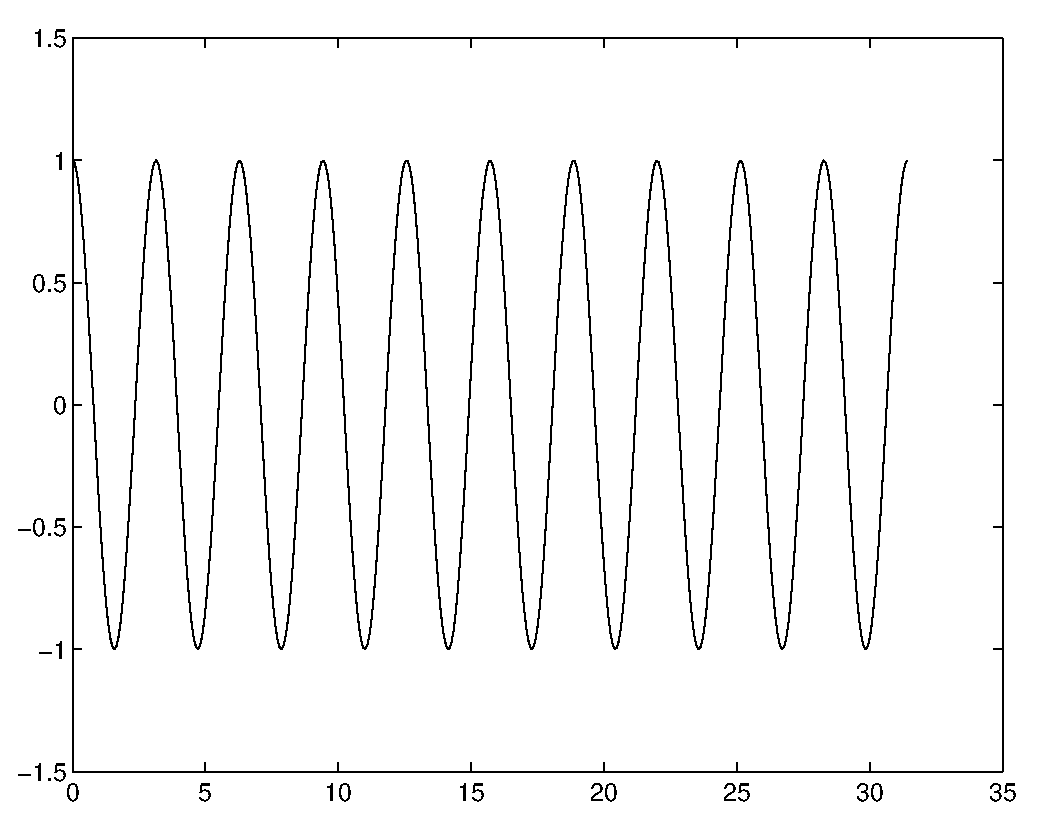
\psfig{file=figures/reson1a.eps,width=3.0in}
           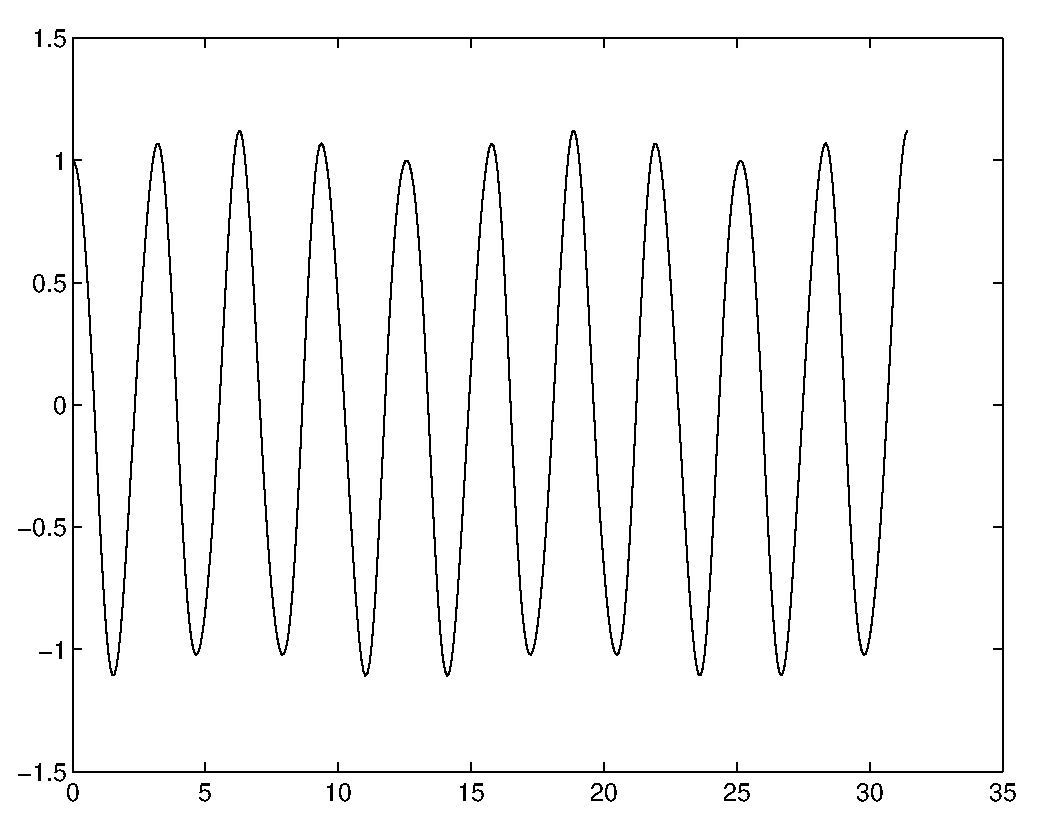
\psfig{file=figures/reson1b.eps,width=3.0in}}
           \caption{Solutions to: (Left) the unforced undamped spring
        equation and (Right) the forced spring equation when $\omega =4.5$.}
           \label{F:nonreson}
\end{figure}

\subsubsection*{Beats}
\index{beats}

Using the trigonometric identity
\[
\cos A - \cos B = -2\sin\left(\frac{A+B}{2}\right)
\sin\left(\frac{A-B}{2}\right),
\]
we find that the solution $x(t)$ is approximately
\begin{equation}  \label{e:x(t)reson3}
x(t) \approx  \frac{1}{1-\omega^2} (\cos(\omega t)-\cos(t))=
\frac{2}{\omega ^2-1}
\sin\left(\frac{\omega+1}{2}t\right)\sin\left(\frac{\omega-1}{2}t\right)
\end{equation}
when $\omega$ is close to $1$.  Note that the first sine term on the right hand
side of \Ref{e:x(t)reson3} has period about $2\pi$ while the second sine term 
has a large period of $4\pi/(\omega-1)$.  For example, when $\omega=1.05$, this
fact leads to periodic behavior of period about $2\pi$ and a 
modulation\index{modulation} 
of period about $80\pi$.  See Figure~\ref{F:beats}.
\begin{figure}[htb]
           \centerline{%
           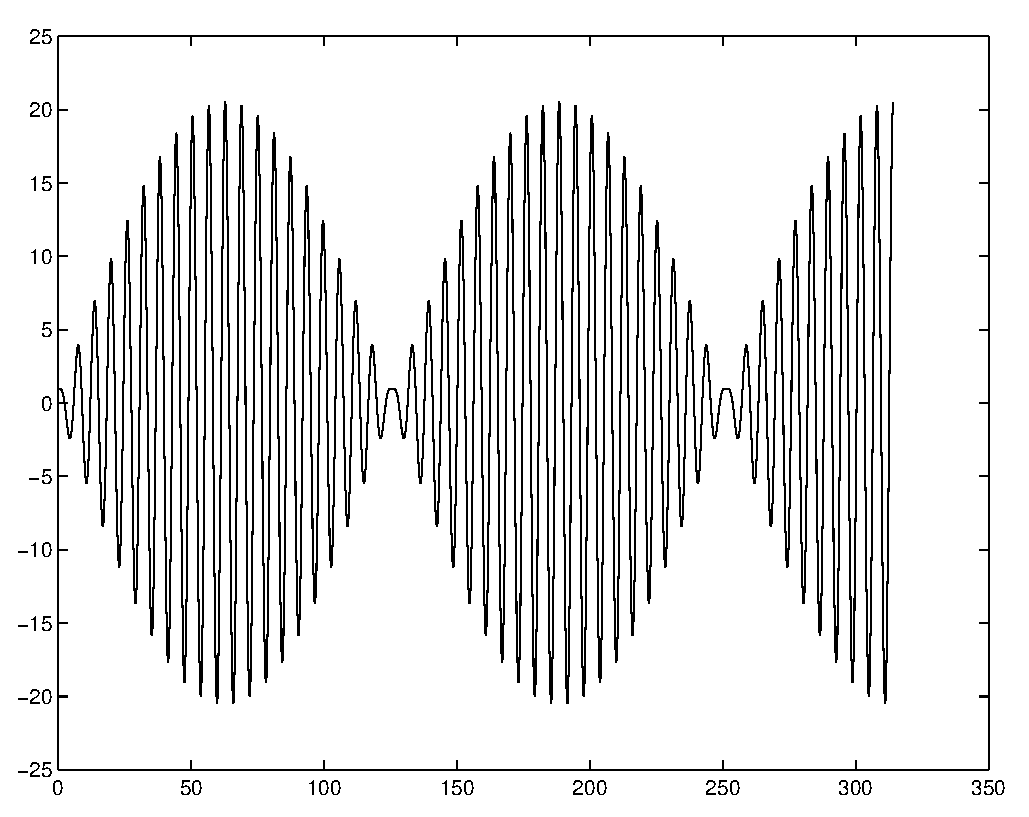
\psfig{file=figures/beats.eps,width=3.5in}}
           \caption{Beats in the solution $x(t)$ to \protect{\Ref{e:x(t)reson}} 
		when $\omega =1.05$ and $0\leq t\leq 100\pi$.}
           \label{F:beats}
\end{figure}  \index{beats}

\subsubsection*{Resonance}
\index{resonance}

When $\omega = 1$ it follows from \Ref{eq:uspfsoln} that every
solution to \Ref{eq:uspf} is unbounded as $t$ goes to infinity.  This
phenomenon is called {\em resonance\/}, and is due to the fact that the
internal frequency\index{frequency!internal} is the same as the 
forcing frequency\index{frequency!forcing}.  The solution
to \Ref{eq:uspf} for $\omega=1$ is shown in Figure~\ref{F:reson} (right).
Resonance shows that when the forcing frequency equals the internal 
frequency, the forcing amplifies the internal dynamics.

Note that when $\omega$ is close to $1$ the solution follows the solution 
for $\omega =1$ for some length of time.  See Figure~\ref{F:reson} where 
the solutions for $\omega =1.05$ and $\omega =1$ are given.  But it is only 
when $\omega =1$ exactly that unbounded growth or resonance actually occurs 
while the nearby solution has long term modulation or beats.
\begin{figure}[htb]
           \centerline{%
           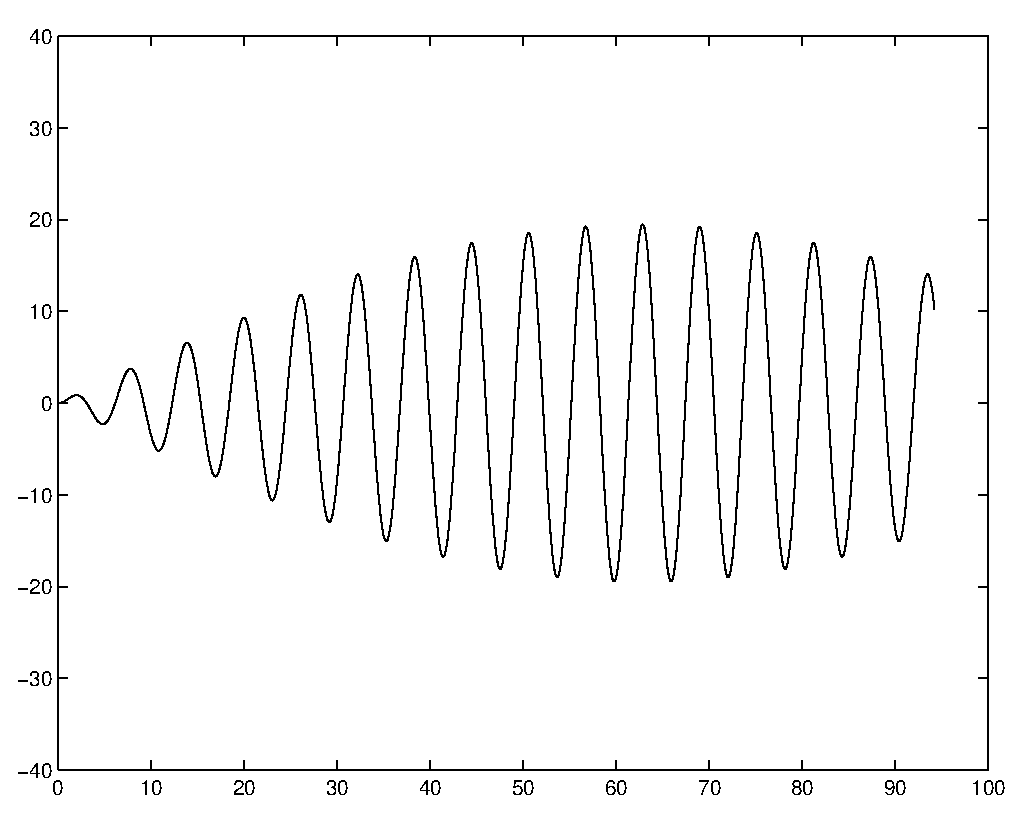
\psfig{file=figures/resona.eps,width=3.5in}
           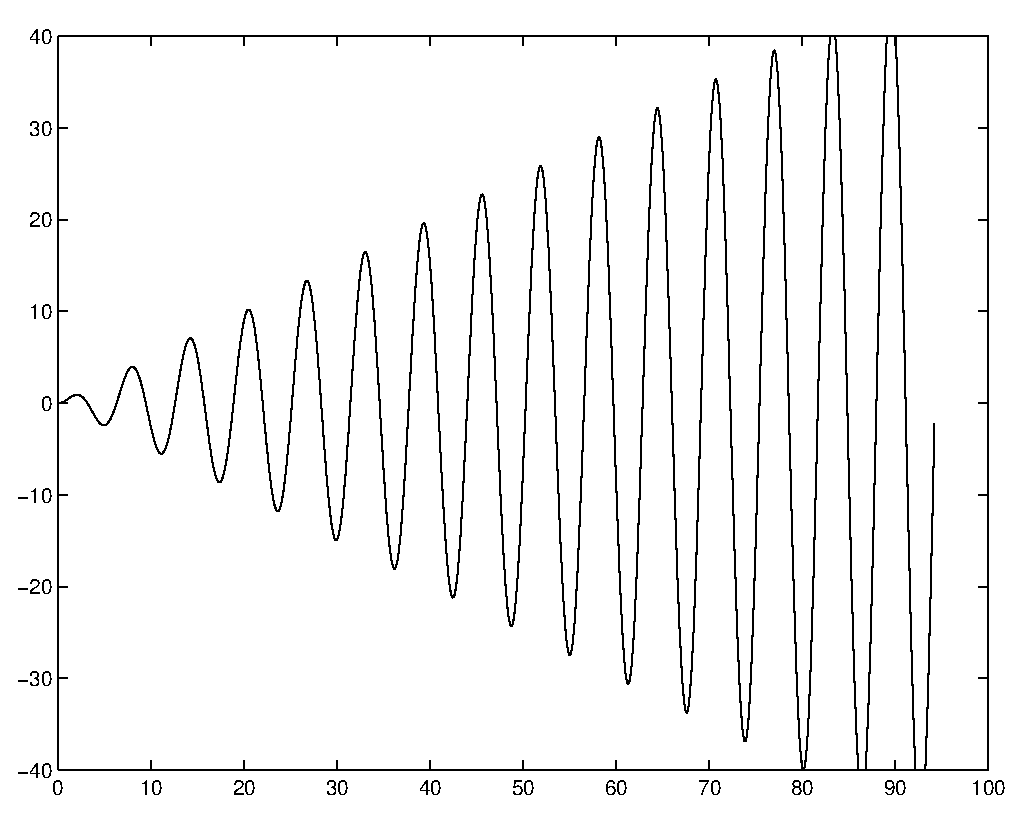
\psfig{file=figures/resonb.eps,width=3.5in}}
           \caption{Two solutions $x(t)$ from \protect{\Ref{e:x(t)reson}} when
                $\omega =1.05$ and $\omega =1$ for $0\leq t\leq 30\pi$.}
           \label{F:reson}
\end{figure}  \index{resonance}



\EXER

\TEXER


\begin{exercise} \label{c12.5.1}
Consider the following equation for the periodically forced
undamped spring\index{spring!undamped!periodically forced}:
\[
\ddot x + \kappa x = A\cos(\omega t).
\]
(Here the constant of the spring $\kappa$ and the amplitude $A$ of the
forcing are assumed to be positive.)  Determine the general solution of
this equation depending on the constants $\kappa$, $A$ and $\omega $.
{\bf Hint:} Proceed as in the text and distinguish between the two
different cases where $\omega \not=\sqrt{\kappa}$ and 
$\omega =\sqrt{\kappa}$.
\end{exercise}

\begin{exercise} \label{c12.5.2}
The following equation describes the behavior of a damped 
spring\index{spring!damped} that is 
forced periodically\index{forcing!periodic}:
\[
\ddot x + 2\dot x + 2x = \sin(2t).
\]
Find real constants $\gamma$ and $\delta$ so that
\[
x_p(t) = \gamma \cos(2t)+ \delta \sin(2t),
\]
is a particular solution of this second order equation.  Write down the
general solution and discuss the behavior of solutions if time $t$
is going to infinity.
\end{exercise}

\begin{exercise} \label{c12.5.3}
Let $x_\omega(t)$ be the solution to \Ref{eq:uspf} given in 
\Ref{e:x(t)reson}.  Show that 
\[
\lim_{\omega\to 1}x_\omega(t) = x_1(t)
\]
for every real number $t$.
\end{exercise} 

\noindent In Exercises~\ref{c12.5.a} -- \ref{c12.5.d} decide whether or not
beats or even resonance occurs in the given differential equations.
\begin{exercise} \label{c12.5.a}
$\ddot{x} + 4x = \cos(2t).$
\end{exercise}
\begin{exercise} \label{c12.5.b}
$\ddot{x} + 16x = \sin(3.9 t).$
\end{exercise}
\begin{exercise} \label{c12.5.c}
$\ddot{x} + 9x = \cos(t).$
\end{exercise}
\begin{exercise} \label{c12.5.d}
$\ddot{x} + 9x = \cos(-3t).$
\end{exercise}

\begin{exercise}  \label{c12.5.4}
Recall the sinusoidally forced second order equation \Ref{eq:uspf}
\[
\ddot x + x = \cos(\omega t).
\]
The second order differential operator that annihilates $\cos(\omega t)$ is
$q(D)=D^2+\omega^2$.  It follows that any solution to \Ref{eq:uspf} must
satisfy the fourth order equation 
\begin{equation} \label{E:ann=res}
q(D)(\ddot x + x)=0.
\end{equation}
Compute the characteristic polynomial of \Ref{E:ann=res} and its roots. Since
the roots typically form two complex conjugate pairs, observe that there is a
connection between the quasiperiodic solutions of this section and those of
Section~\ref{S:NLD}.  What is the special property of these roots that leads
to resonance and why?
\end{exercise}


